%%=============================================================================
%% Methodologie
%%=============================================================================

\chapter{\IfLanguageName{dutch}{Methodologie}{Methodology}}
\label{ch:methodologie}

%% TODO: Hoe ben je te werk gegaan? Verdeel je onderzoek in grote fasen, en
%% licht in elke fase toe welke stappen je gevolgd hebt. Verantwoord waarom je
%% op deze manier te werk gegaan bent. Je moet kunnen aantonen dat je de best
%% mogelijke manier toegepast hebt om een antwoord te vinden op de
%% onderzoeksvraag.


\section{\IfLanguageName{dutch}{Installatie}{Installation}}
\label{sec:M-installatie}

De eerste stap om dit onderzoek uit te voeren is het installeren van de correcte software. Hieronder wordt een overzicht van de delen binnen de installatie getoond:
\begin{itemize}
    \item Hardware
    \item Android Studio
    \item Xcode
    \item JDK
\end{itemize}
Binnen dit deel van de methodologie zullen per deel de vereiste stappen besproken worden om de software te installeren.

    \subsection{\IfLanguageName{dutch}{Hardware}{Hardware}}
    \label{sec:I-hardware}
    Voor de installatie van deze software is het belangrijk te weten dat een computer of laptop die draait op macOS\footnote{apple.com/benl/macos}noodzakelijk is. Hierbij is het ook belangrijk te controleren dat de geïnstalleerde versie minstens macOs Big Sur\footnote{apple.com/benl/macos/big-sur} 11.3.1 is. Dit zal later van belang zijn gezien de testen gedraaid worden op emulators met  iOS 14.3\footnote{apple.com/benl/ios/ios-14} en hiervoor macOS 11.3.1 vereist is. De software kan echter ook geïnstalleerd worden op een computer of laptop die draait op Windows\footnote{microsoft.com/nl-be/windows} maar dan kunnen geen applicaties, noch native noch cross-platform, gemaakt worden voor iOS\footnote{apple.com/benl/ios}.
    \\ \\
    Een ander belangrijk gegeven is dat nog niet alle software, voornamelijk Android Studio\footnote{developer.android.com/studio}, de laatste Apple Silicon\footnote{developer.apple.com/documentation/apple-silicon} processors niet ondersteunen. Een eventuele omweg kan gebeuren via Apple Rosetta 2\footnote{developer.apple.com/documentation/apple-silicon/about-the-rosetta-translation-environment} maar dit lost niet alle problemen op. Indien er toch op een Apple Silicon toestel gewerkt zou willen worden, wordt er aanbevolen de websites van de desbetreffende software te controleren voor compatibiliteit.  
    \\ \\
    Voor dit onderzoek zal dus ook een laptop gebruikt worden die draait op macOs. Het toestel in kwestie is een MacBook Pro 16 inch uit 2019.
    Meer technische informatie over dit toestel kan op volgende link teruggevonden worden:\\
    \verb*|https://support.apple.com/kb/SP809|
    \\ \\
    Meer informatie over de recentste versies van \textbf{macOS Big Sur} kan teruggevonden worden op volgende link:\\
    \verb*|https://support.apple.com/en-us/HT211896|

    \subsection{\IfLanguageName{dutch}{Android Studio}{Android Studio}}
    \label{sec:I-AS}
    Android Studio is het eerste deel van de vereiste software, deze software wordt aangeboden door JetBrains\footnote{jetbrains.com} en door Google\footnote{about.google} als software voor de ontwikkeling van Android\footnote{android.com} applicaties. Android Studio is gebaseerd op IntelliJ IDEA\footnote{jetbrains.com/idea} van JetBrains. De laatste stabiele versie van Android Studio voor macOS is 4.2.  Afhankelijk van het project dat gebruikt wordt, kunnen er echter nog enkele problemen optreden met de versie van Android Jetpack\footnote{developer.android.com/jetpack}. Dit kan opgelost worden door de Canary build van Android studio te downloaden. De laatste versie van Android Studio Canary build\footnote{developer.android.com/studio/preview} is Artic Fox (2020.3.1) Canary 15.
    \\ \\
    De laatste versie van \textbf{Android Studio} kan hier teruggevonden worden:\\
    \verb*|https://developer.android.com/studio|
    \\ \\ 
    De laatste versie van \textbf{Android Studio Canary build} kan hier teruggevonden worden:\\
    \verb*|https://developer.android.com/studio/preview|
    \\ \\
    Oudere versies van Android Studio ondersteunen de recentste plug-ins voor Kotlin Multiplatform Mobile (KMM) niet. Hierbij is het dus belangrijk dat de versie die geïnstalleerd wordt 4.2 of recenter is.
    \\ \\ 
    Tijdens de installatie zal Android Studio kan er best geopteerd worden on de standaard instellingen te nemen. Daarnaast zullen verschillende zaken geinstalleerd worden namelijk:
    \begin{itemize}
        \item Android Emulator
        \item Android SDK Build Tools 30.0.3
        \item Android SDK Platform 30
        \item Android SDK Platform-Tools
        \item Android SDK Tools
        \item Google APIs Intel x86 Atom System Image
        \item Intel x86 Emulator Accelerator (HAXM installer)
        \item SDK Patch Applier v4
        \item Sources for Android 30
    \end{itemize}
    Deze zijn allemaal van belang voor zowel de native Android ontwikkeling als de KMM cross-platform ontwikkeling. Eens de installatie voltooid is kan via de AVD manager een emulator geïnstalleerd worden. Voor deze studie zal er een Pixel 4a\footnote{store.google.com/us/product/pixel\_4a?hl=en-US} geïnstalleerd worden met Android 11\footnote{android.com/android-11} (API Level 30). Deze emulator zal gebruikt worden voor de native Android en de KMM cross-platform applicatie te testen. Eens deze emulator correct is geïnstalleerd kan deze teruggevonden worden in de ADV Manager zoals op figuur \ref{fig:M-as-adv-manager}
    \begin{figure}
        \centering
        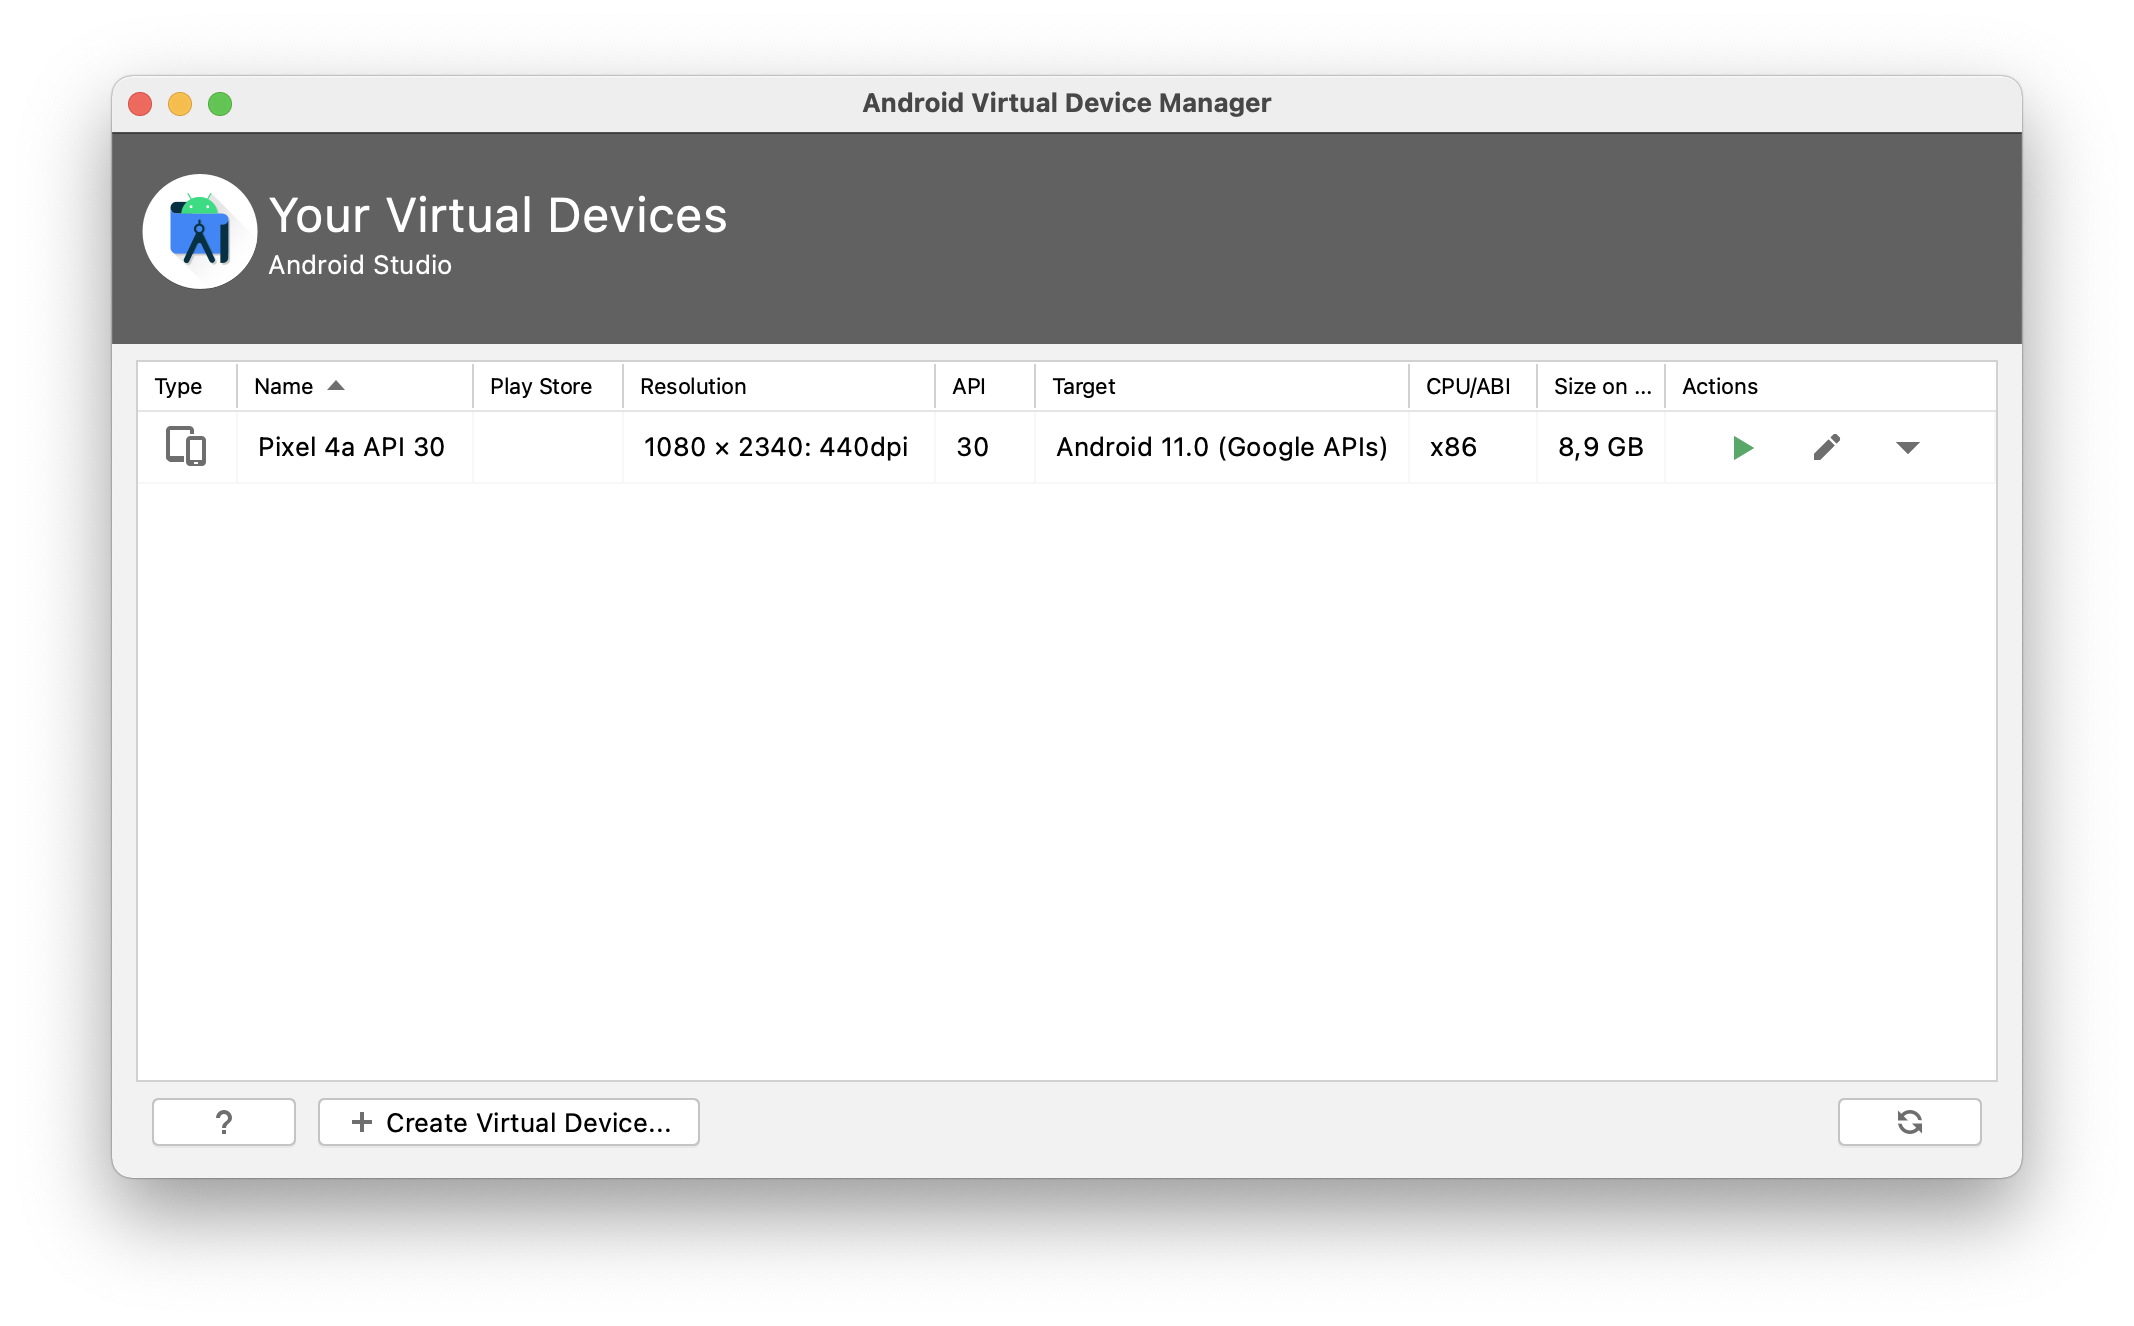
\includegraphics[width=10cm]{img/as-adv-manager.png}
        \caption{De ADV Manager in Android Studio met de Pixel 4a emulator geïnstalleerd}
        \label{fig:M-as-adv-manager}
    \end{figure}
    \\ \\
    Zoals net vermeld is het ook nodig om de KMM plug-in te installeren voor Android Studio. De plug-in maakt het mogelijk om KMM projecten aan te maken. Hierdoor kan de business logica geschreven worden voor beide platformen, gedeeld of per platform. Een andere feature van de plug-in is dat de iOS applicatie kan gestart en gedebugd worden vanuit Android Studio. Daarnaast zullen de gebruikers door de plug-in ook de mogelijkheid krijgen om nieuwe KMM applicaties aan te maken.
    \\ \\ 
    De laatste versie van de \textbf{KMM plug-in} kan hier teruggevonden worden:\\
    \verb*|https://plugins.jetbrains.com/plugin/14936-kotlin-multiplatform-mobile|
    
    Onderstaande figuren tonen het proces om een nieuwe KMM applicatie te maken aan de hand van de KMM plug-in. 
    \begin{itemize}
        \item Figuur \ref{fig:M-kmm-plugin-1} toont de mogelijke opties binnen Android Studio voor het aanmaken van een nieuw project, eens de plugin correct is geïnstalleerd, zal daar ook de optie  `KMM Application’ beschikbaar zijn.
        \item Figuur \ref{fig:M-kmm-plugin-2} toont de standaard instellingen voor een KMM project, deze instellingen lopen gelijk met de standaard instellingen voor een standaard Android project.
        \item Figuur \ref{fig:M-kmm-plugin-3} toont de mogelijkheden om de verschillende delen van de KMM te benoemen, standaard zullen hier de waarden androidApp, iosApp en shared staan. Daarnaast kunnen deze delen nog een beschrijving krijgen. Als laatste is er de optie om templates voor testen toe te voegen aan de shared module.
    \end{itemize}
 
    \begin{figure}
        \centering
        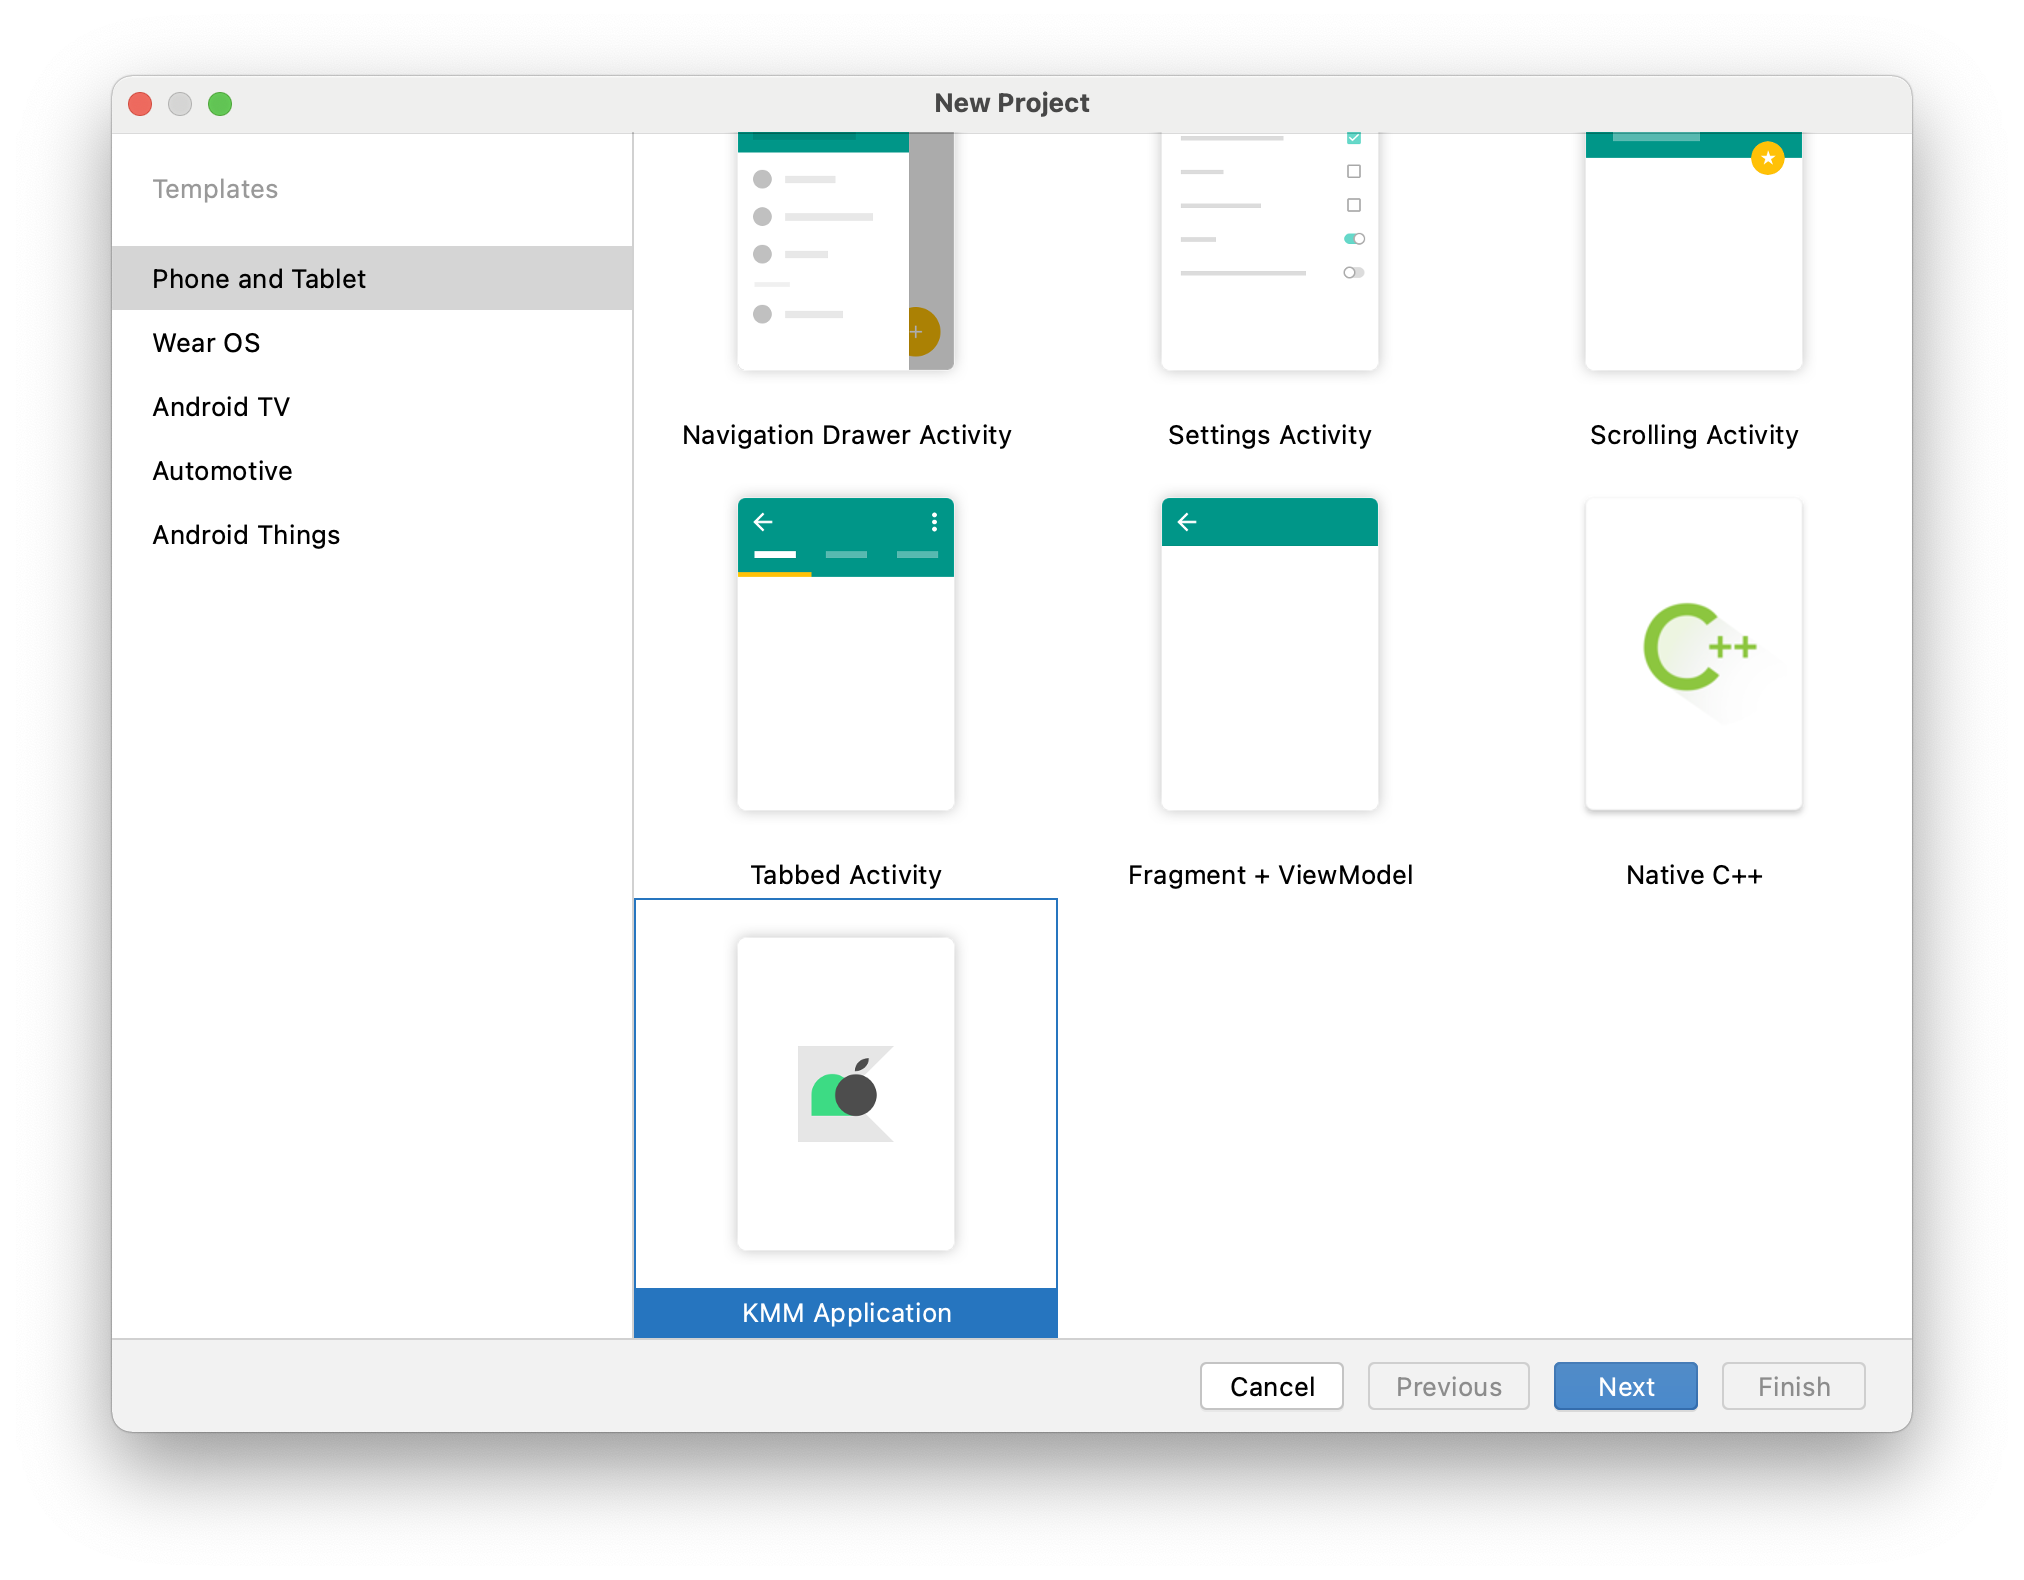
\includegraphics[width=10cm]{img/kmm-plugin-1.png}
        \caption{De opties voor een nieuw project binnen Android Studio, hierbij is een KMM applicatie ook beschikbaar}
        \label{fig:M-kmm-plugin-1}
    \end{figure}
    \begin{figure}
        \centering
        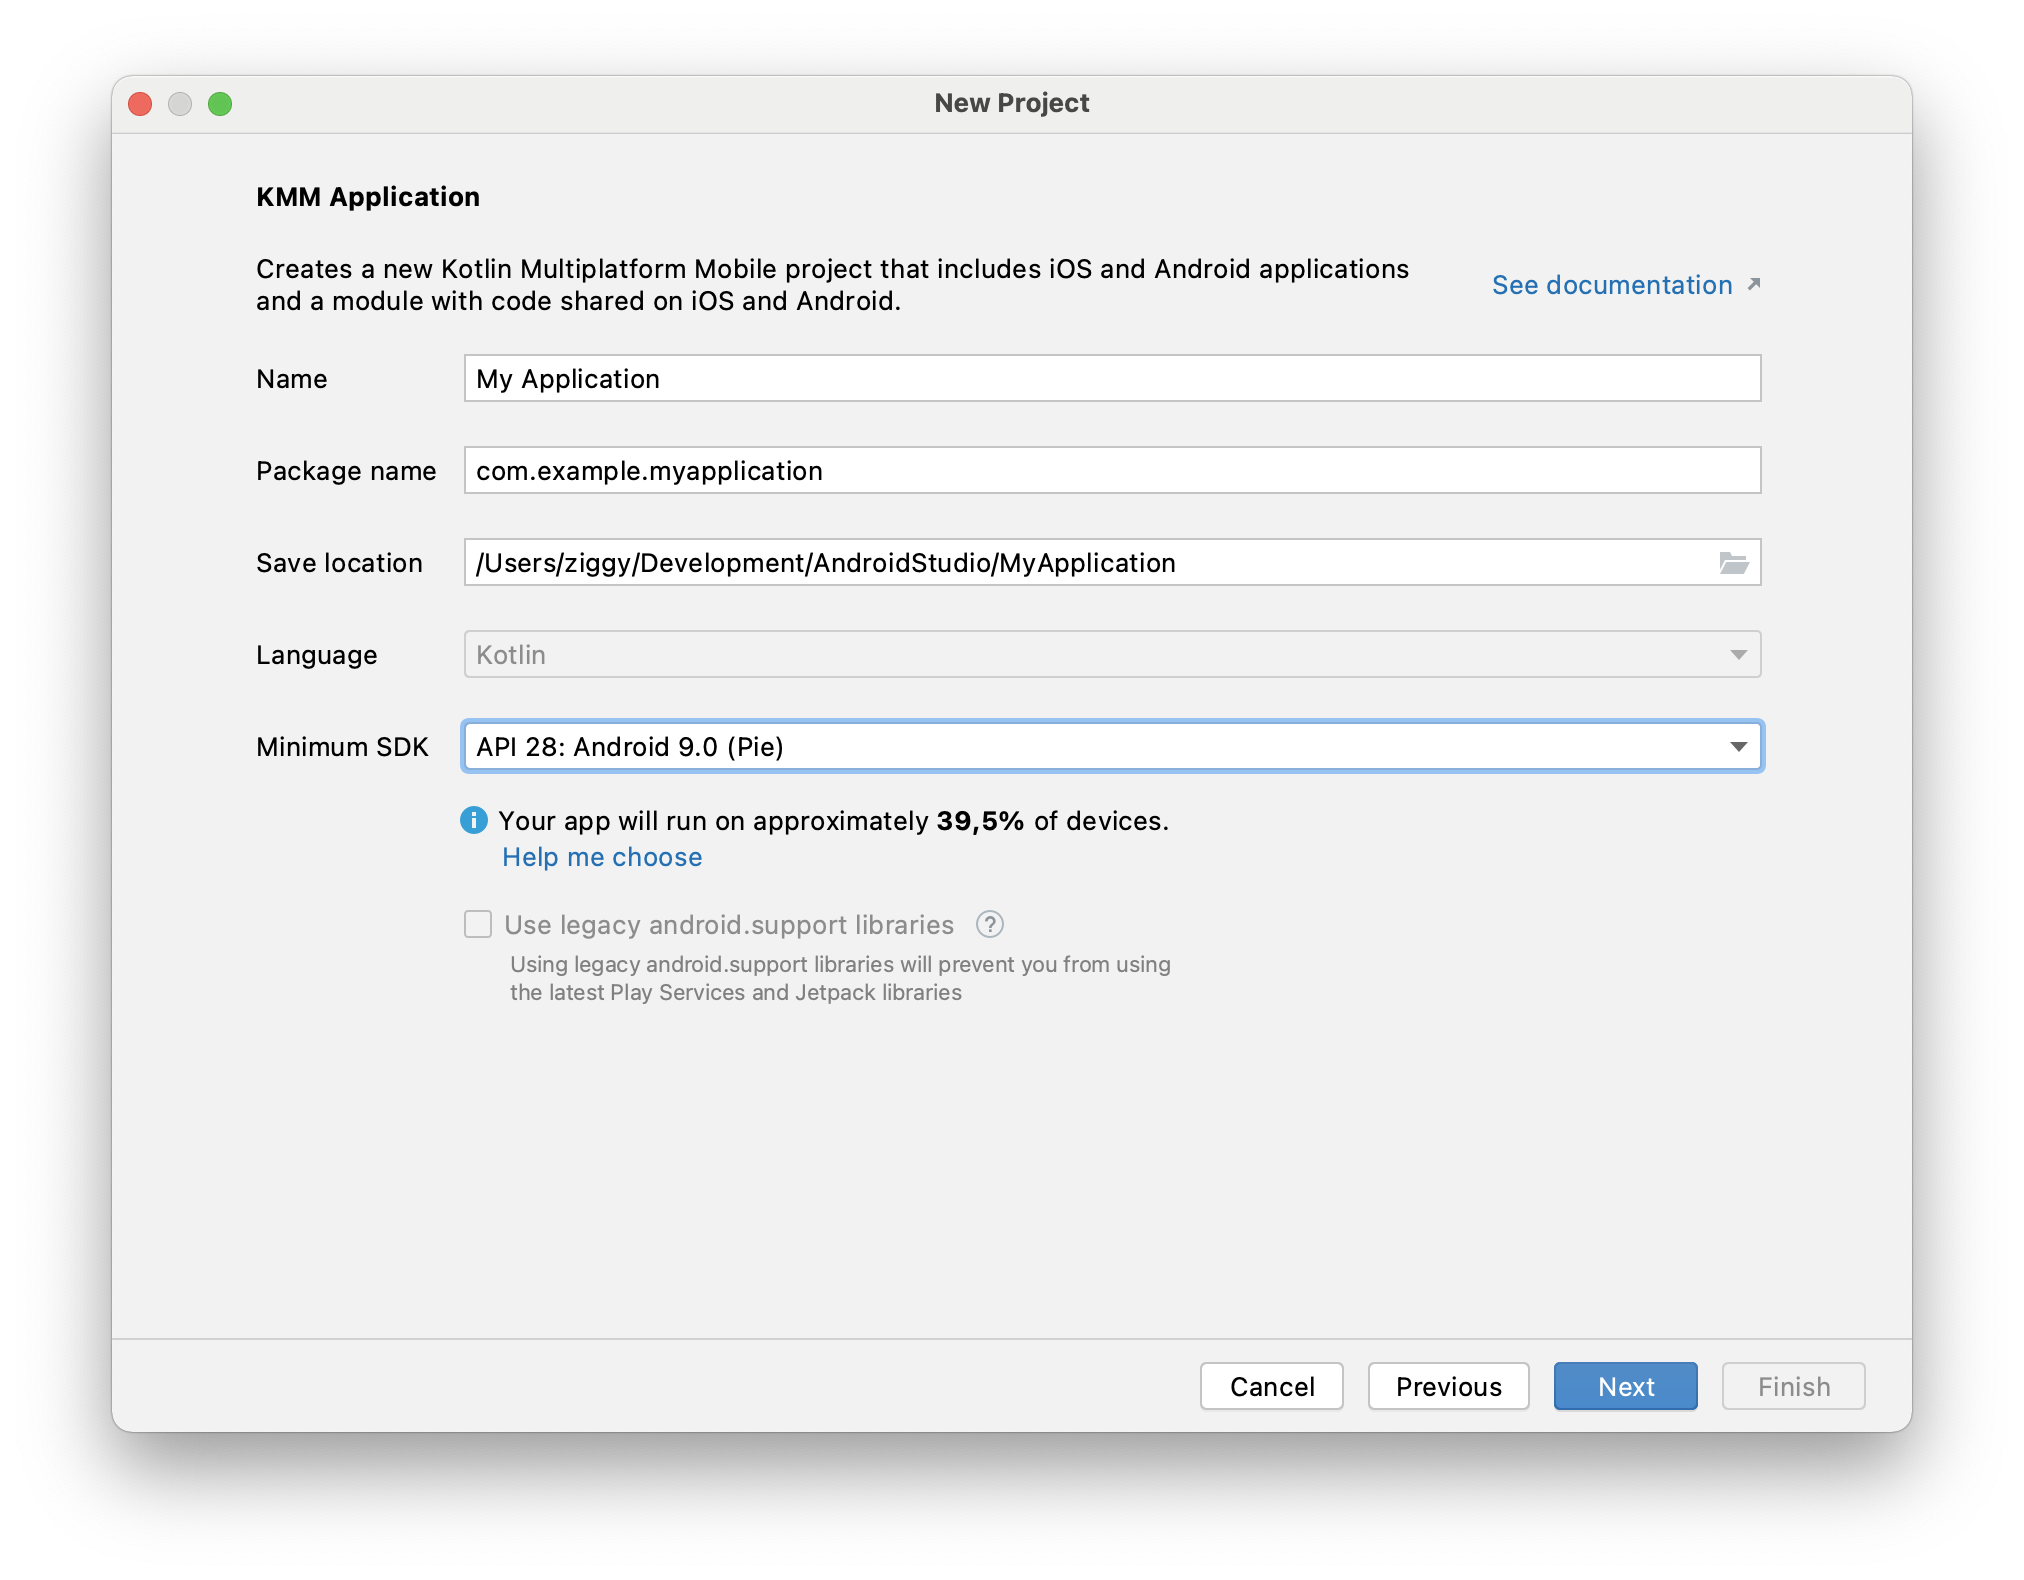
\includegraphics[width=10cm]{img/kmm-plugin-2.png}
        \caption{De standaard instellingen voor een KMM project}
        \label{fig:M-kmm-plugin-2}
    \end{figure}
    \begin{figure}
        \centering
        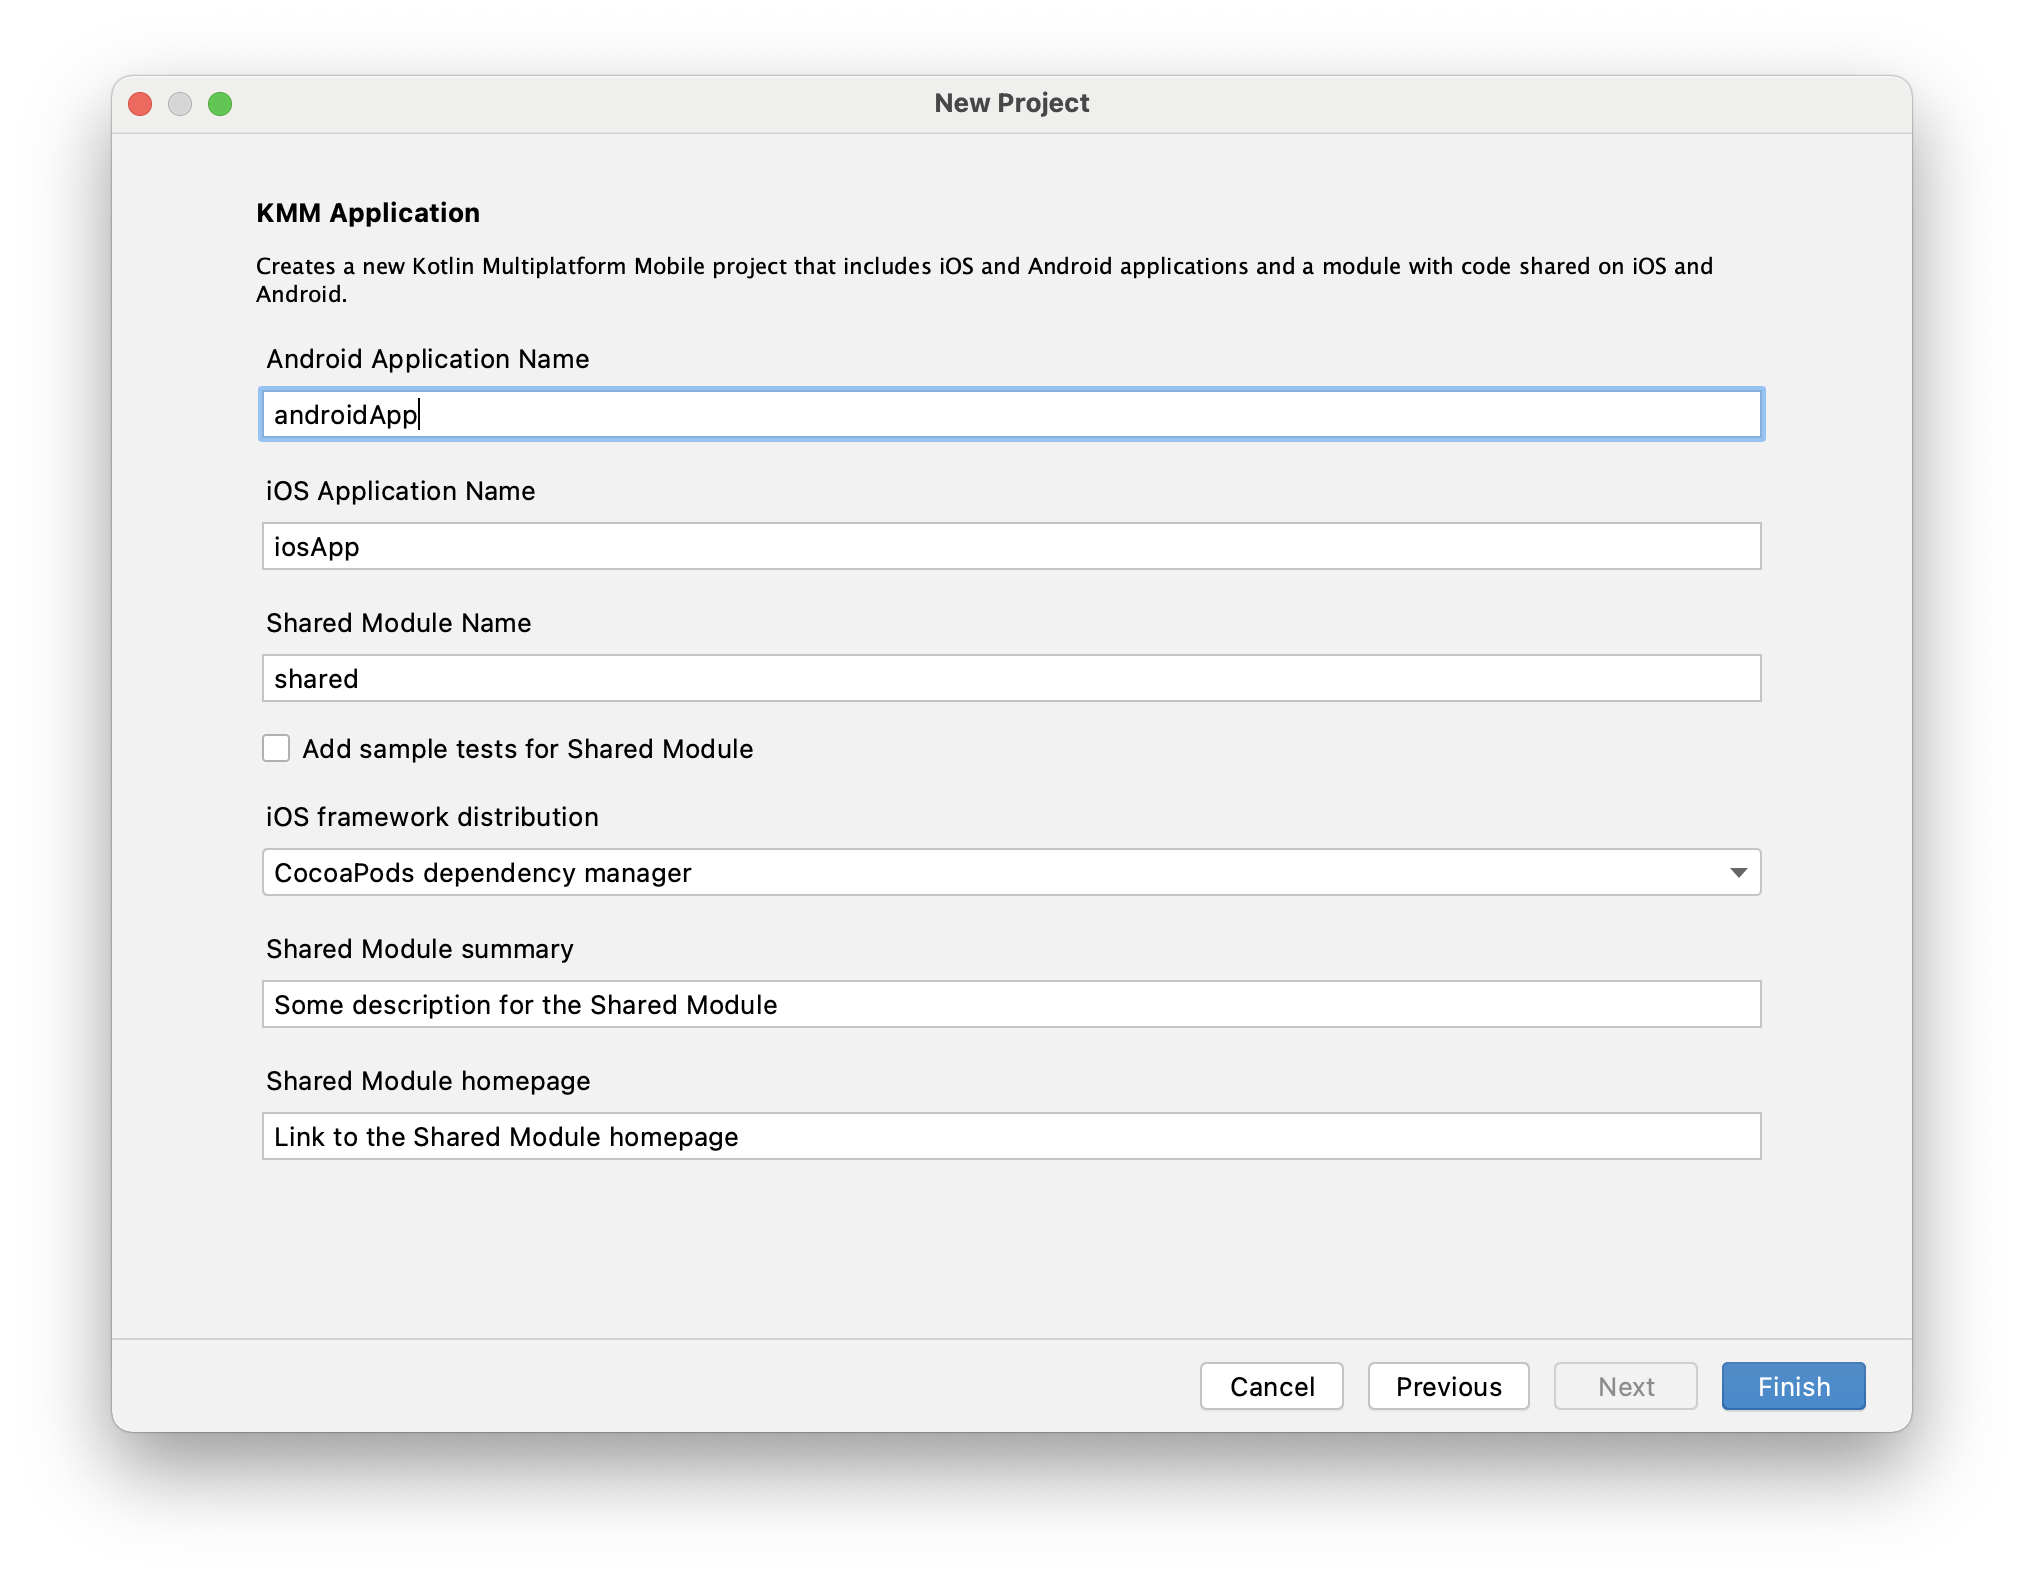
\includegraphics[width=10cm]{img/kmm-plugin-3.png}
        \caption{De instellingen van een KMM project voor de gedeelde logica en de native iOS en Android delen}
        \label{fig:M-kmm-plugin-3}
    \end{figure}

    Indien er problemen zouden zijn met de KMM plug-in kan er via de instellingen van Android Studio gecontroleerd worden of de plug-in goed geïnstalleerd is en actief staat.
    \\ \\
    Android Studio -> Voorkeuren -> Plugins -> Kotlin Multiplatform Mobile
    \\ \\
    De plug-in zou bij de geïnstalleerde plug-ins moeten staan en moet actief staan.
    \begin{figure}
        \centering
        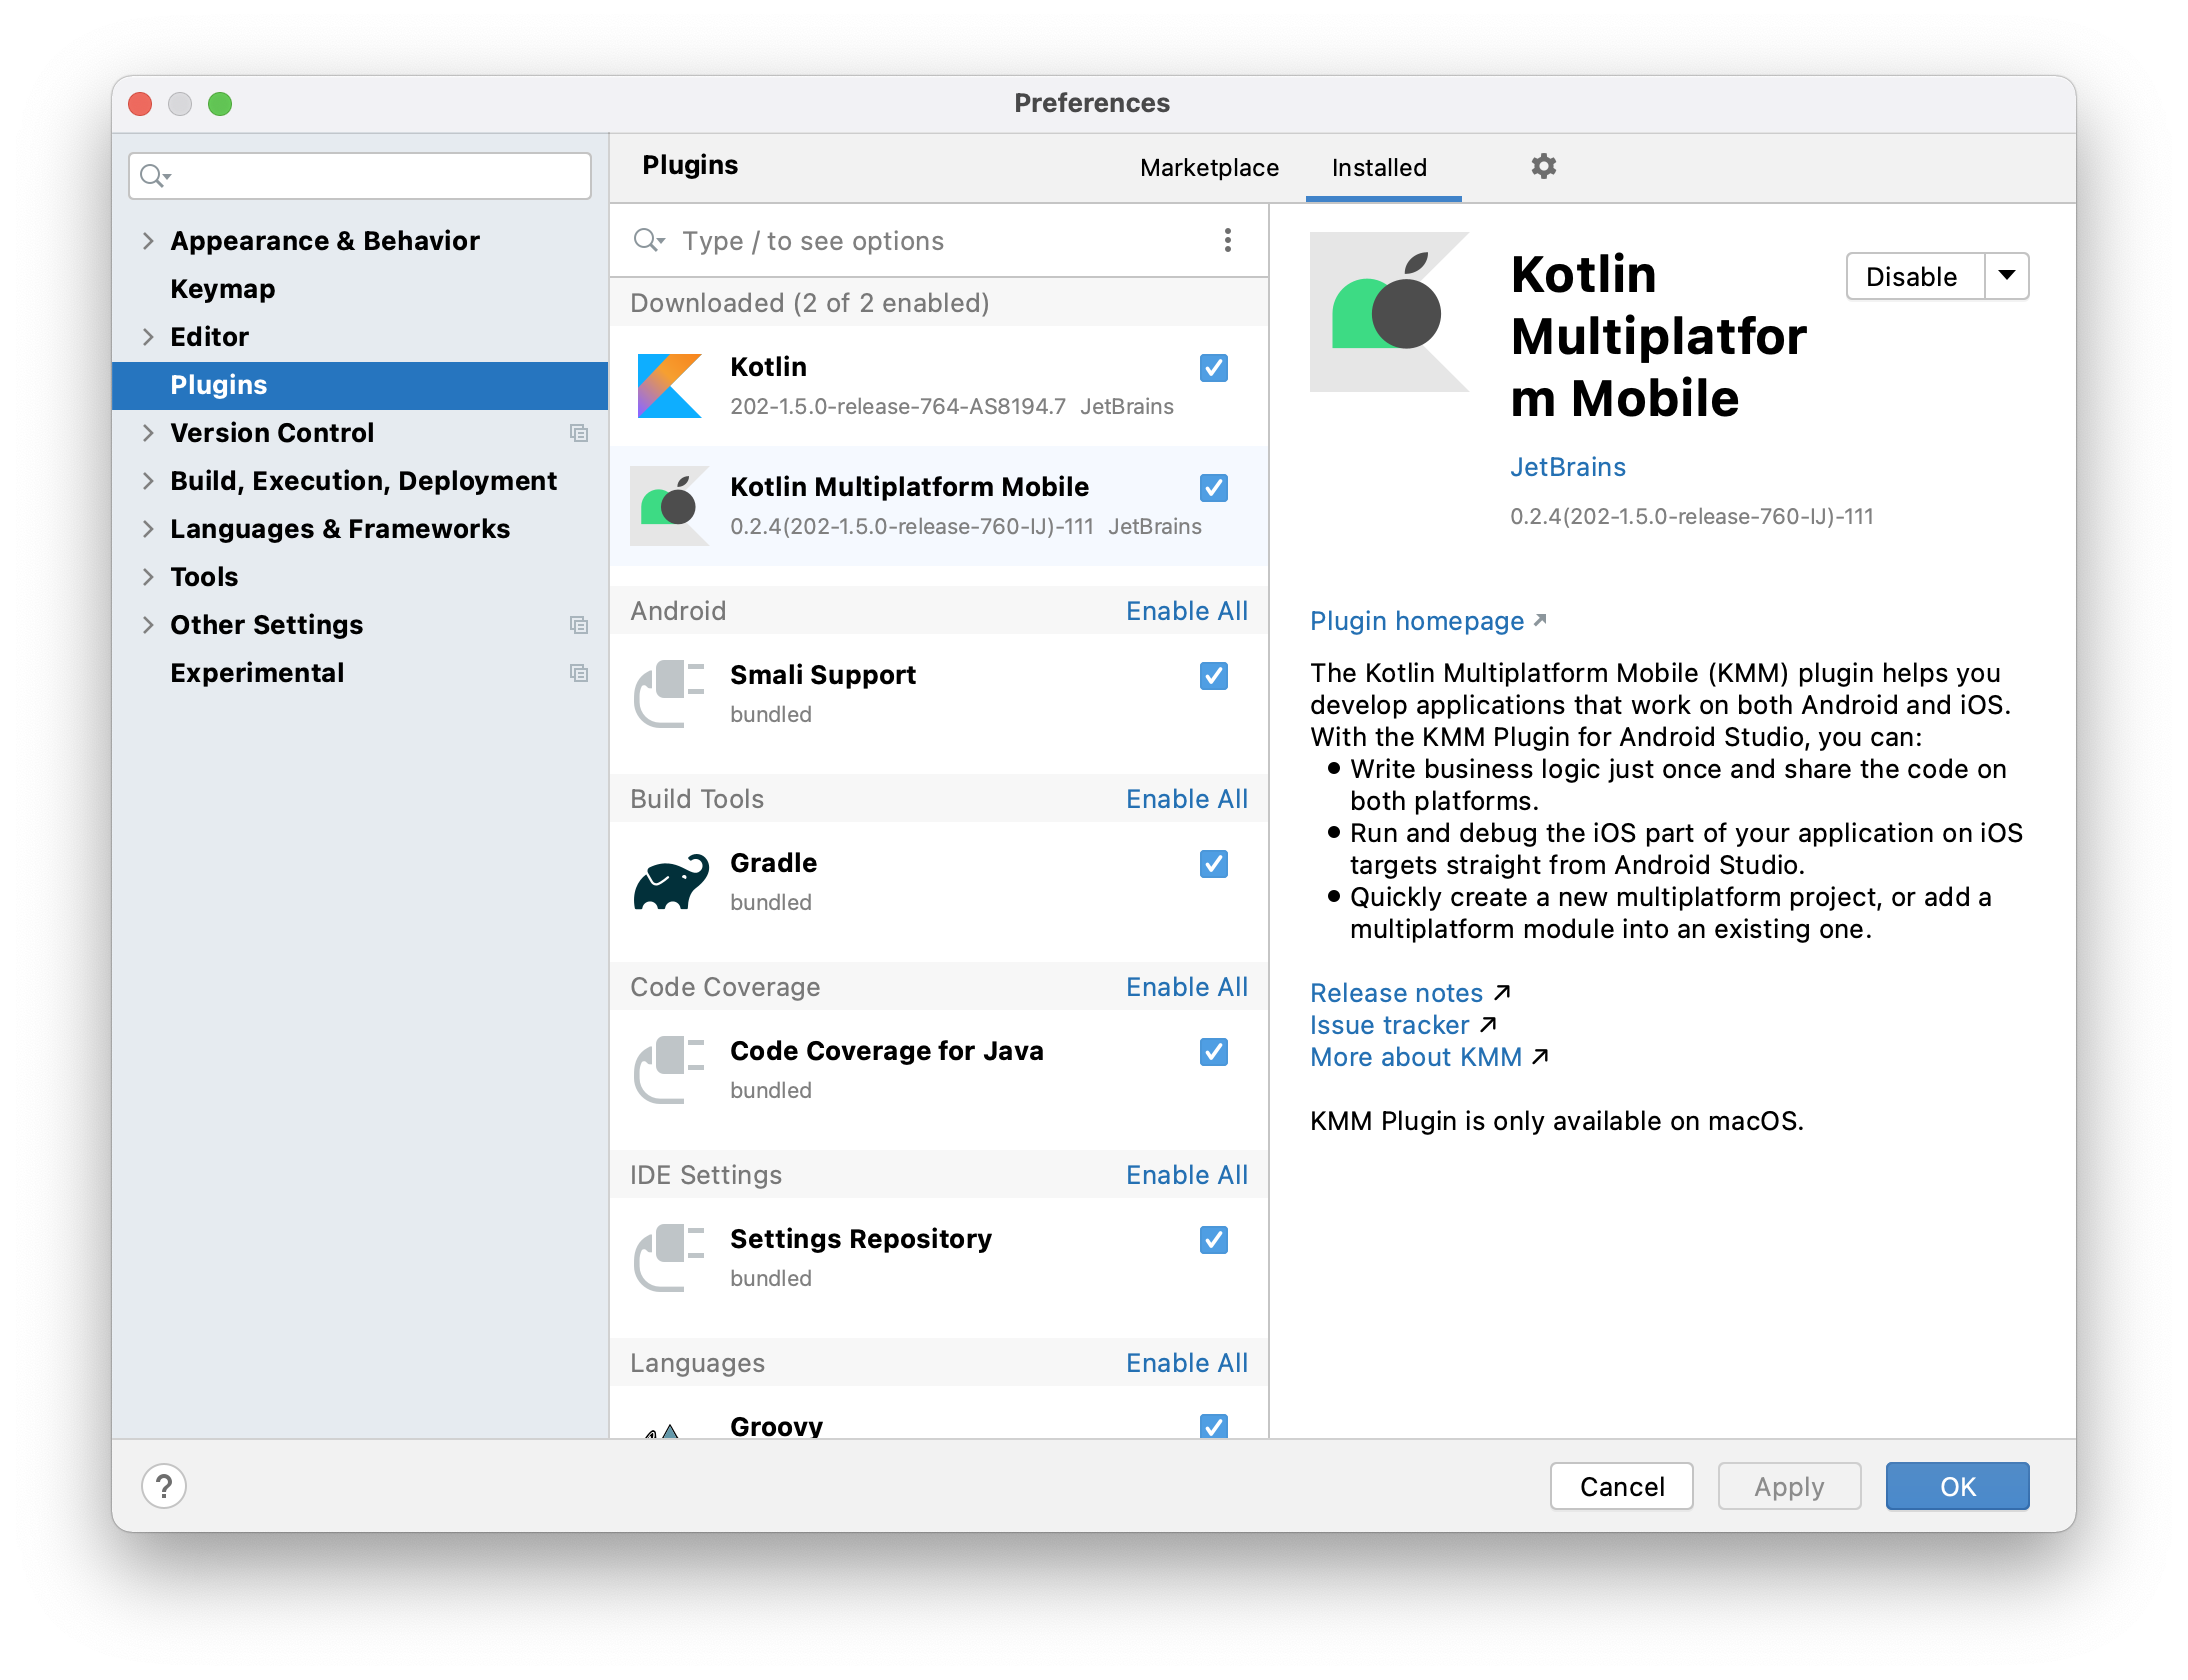
\includegraphics[width=10cm]{img/kmm-plugin-4.png}
        \caption{De plug-in geïnstalleerd binnen Android Studio}
        \label{fig:M-kmm-plugin-4}
    \end{figure}
   
   
    \subsection{\IfLanguageName{dutch}{Xcode}{Xcode}}
    \label{sec:I-Xcode}
    Het tweede deel van software dat dient geïnstalleerd te worden is Xcode\footnote{developer.apple.com/xcode}, de softwareontwikkeling omgeving van Apple\footnote{apple.com} voor toestellen die draaien op iOS, iPadOS\footnote{apple.com/benl/ipados}, macOS...  Deze software is uitsluitend beschikbaar voor toestellen die draaien op macOS. De laatste beschikbare versie is Xcode 12.5, deze ondersteunt het bouwen applicaties tot iOS 14.3, iPadOS 14.3\footnote{apple.com/benl/ipados/ios-14}, watchOS 7.4\footnote{apple.com/benl/watchos/watchos-7}... 
    \\ \\ 
    De laatste versie van \textbf{Xcode} kan geïnstalleerd worden via de Apple Developer website of via de App Store\footnote{apple.com/benl/app-store} op macOS: \\
    \verb*|https://developer.apple.com/xcode/|
    \\
    \verb*|https://apps.apple.com/nl/app/xcode/id497799835?mt=12|
    \\ \\ 
    Naast Xcode zal voor deze studie ook gebruik gemaakt worden van Xcode Command Line Tools, deze komen normaal standaard mee met de Xcode IDE. Indien de Xcode Command Line Tools niet geïnstalleerd zouden zijn kan dit via volgend terminal commando gedaan worden. \\
    \begin{lstlisting}
        //Terminal.app
        xcode-select --install
    \end{lstlisting}
    Eens deze installatie voltooid is dient er nog binnen Xcode een aanpassing gemaakt te worden zodat de Command Line Tools actief zijn. Via Xcode -> Voorkeuren -> Locaties, moeten de Command Line Tools ingesteld worden op `Xcode 12.5 (12E262)' deze optie zou beschikbaar moeten zijn in de selectielijst. Figuur \ref{fig:M-xcode-locations} toont het instellingenmenu voor Locaties met de correcte waarden. 
    \begin{figure}
        \centering
        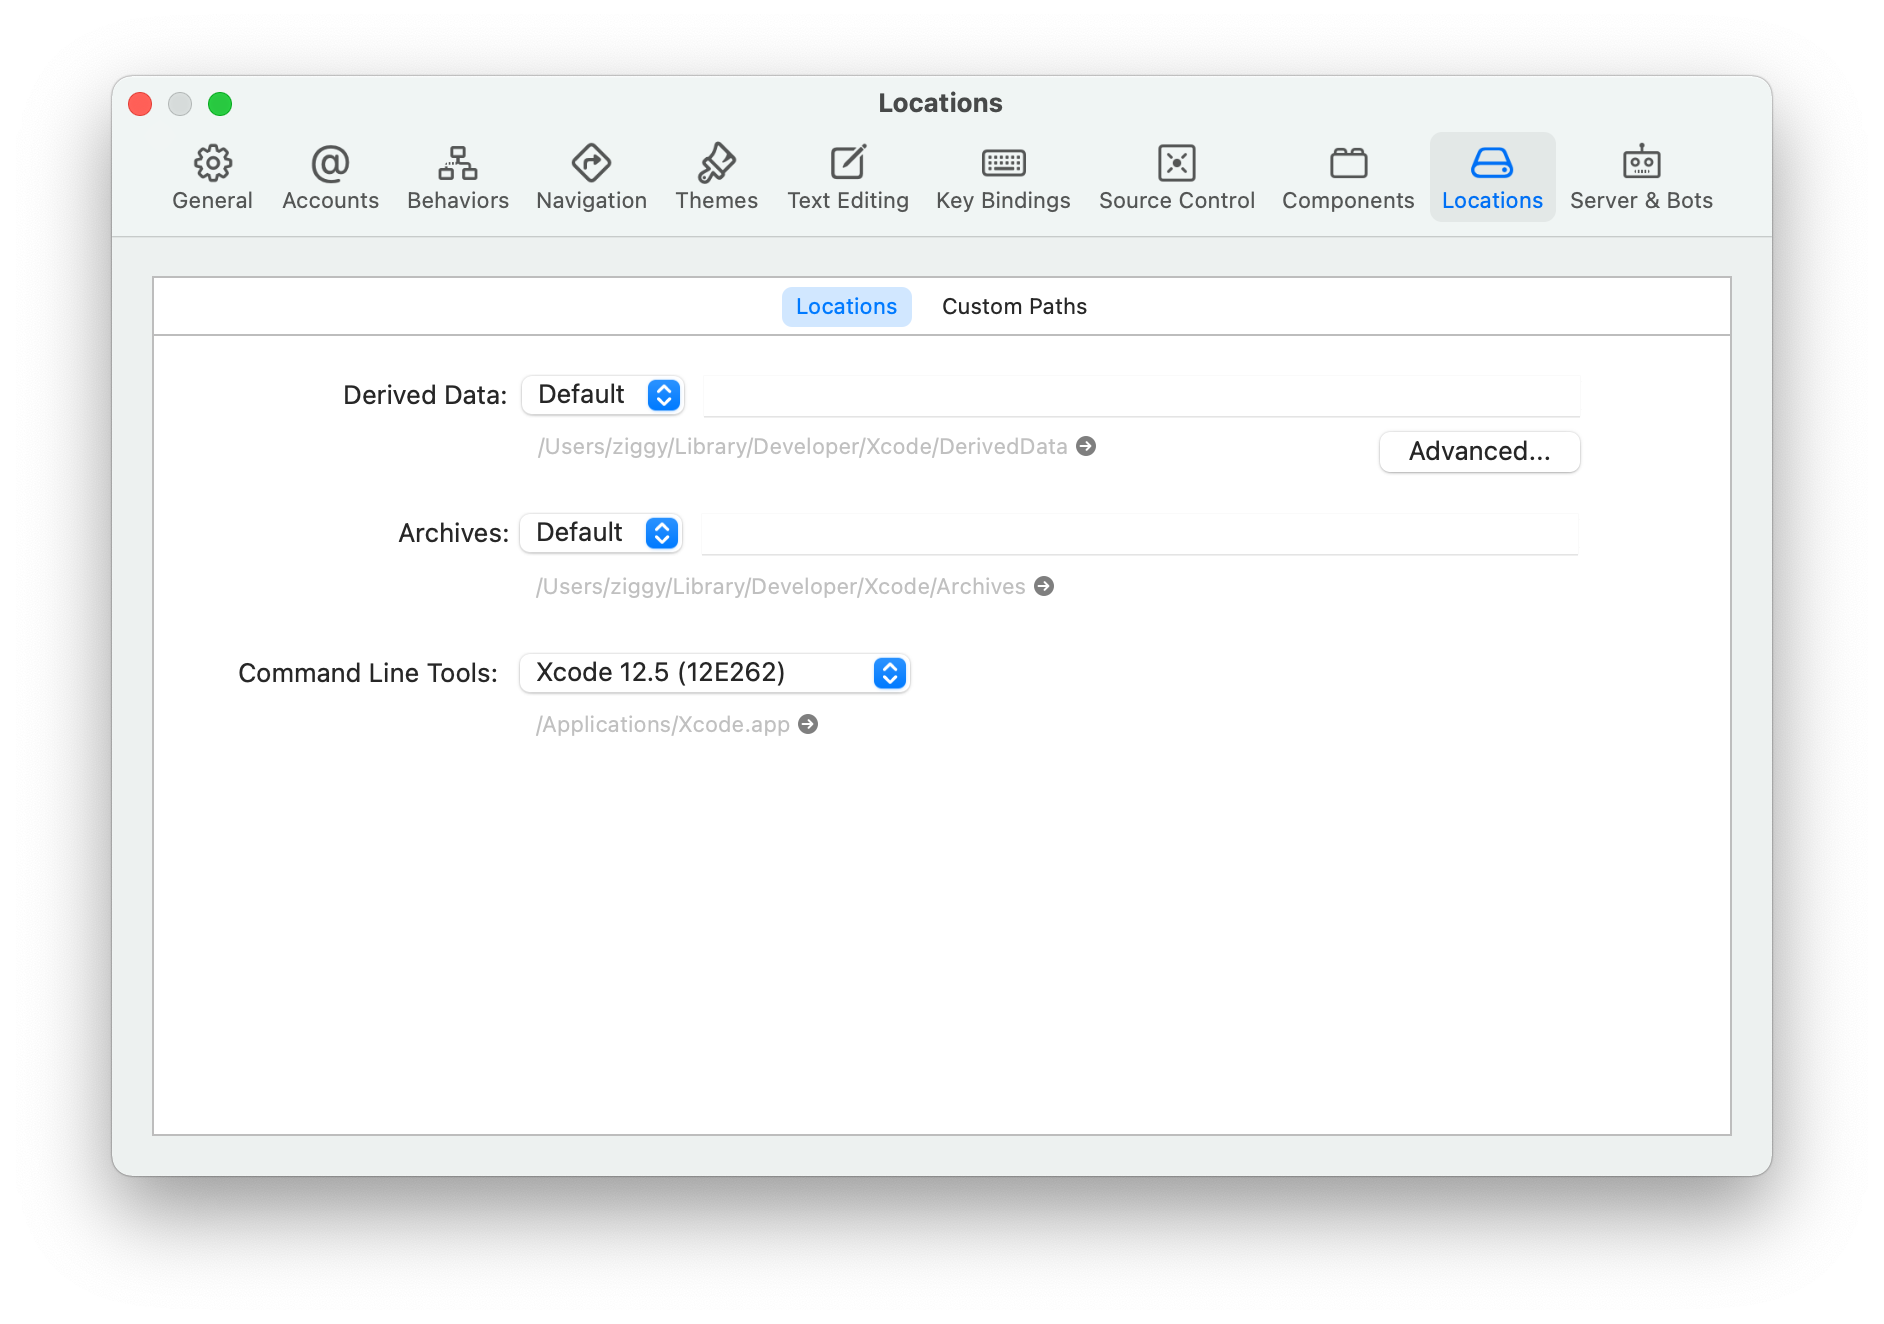
\includegraphics[width=10cm]{img/xcode-locations}
        \caption{De Xcode Command Line Tools correct geconfigureerd binnen Xcode}
        \label{fig:M-xcode-locations}
    \end{figure}
    
    Tijdens de installatie van Xcode worden alle emulators al voorzien waardoor er hier geen extra instellingen moeten aan gebeuren. Voor deze studie zal gebruik gemaakt worden van een iPhone 12\footnote{apple.com/benl/iphone-12} emulator met iOS 14.3.
    \\ \\
    Naast de installatie van Xcode zal ook CocoaPods geïnstalleerd moeten worden om de KMM plugin correct te laten werken. CocoaPods kan geinstalleerd worden aan de hand van onderstaand commando.
    
    \begin{lstlisting}
        //Terminal.app
        sudo gem install cocoapods
    \end{lstlisting}
    
    \subsection{\IfLanguageName{dutch}{JDK}{JDK}}
    \label{sec:I-JDK}
    De laatste stap van het installatieproces is het installeren van een JDK of Java Development Kit. Voor deze studie zal Java SE 16\footnote{oracle.com/java/technologies/javase-downloads.html} geïnstalleerd worden. Dit is de laatst beschikbare versie van Java\footnote{java.com}. Alle andere versies van Java SE zijn hier terug te vinden \verb*|https://www.oracle.com/java/technologies/oracle-java-archive-downloads.html|
    
    De laatste versie van de \textbf{Java JDK} kan geïnstalleerd worden via volgende website: \\
    \verb*|https://www.oracle.com/java/technologies/javase-jdk16-downloads.html|
    \\
    
    Eens de installatie is voltooid kan de gebruiker controleren of de installatie geslaagd is door onderstaand commando uit te voeren.
    \begin{lstlisting}
        //Terminal.app
        java --version
    \end{lstlisting}
    Indien de installatie geslaagd is en Java SE 16 correct is geïnstalleerd zal de gebruiker volgende output krijgen zoals in figuur \ref{fig:M-jdk-version} 
    
    \begin{figure}
        \centering
        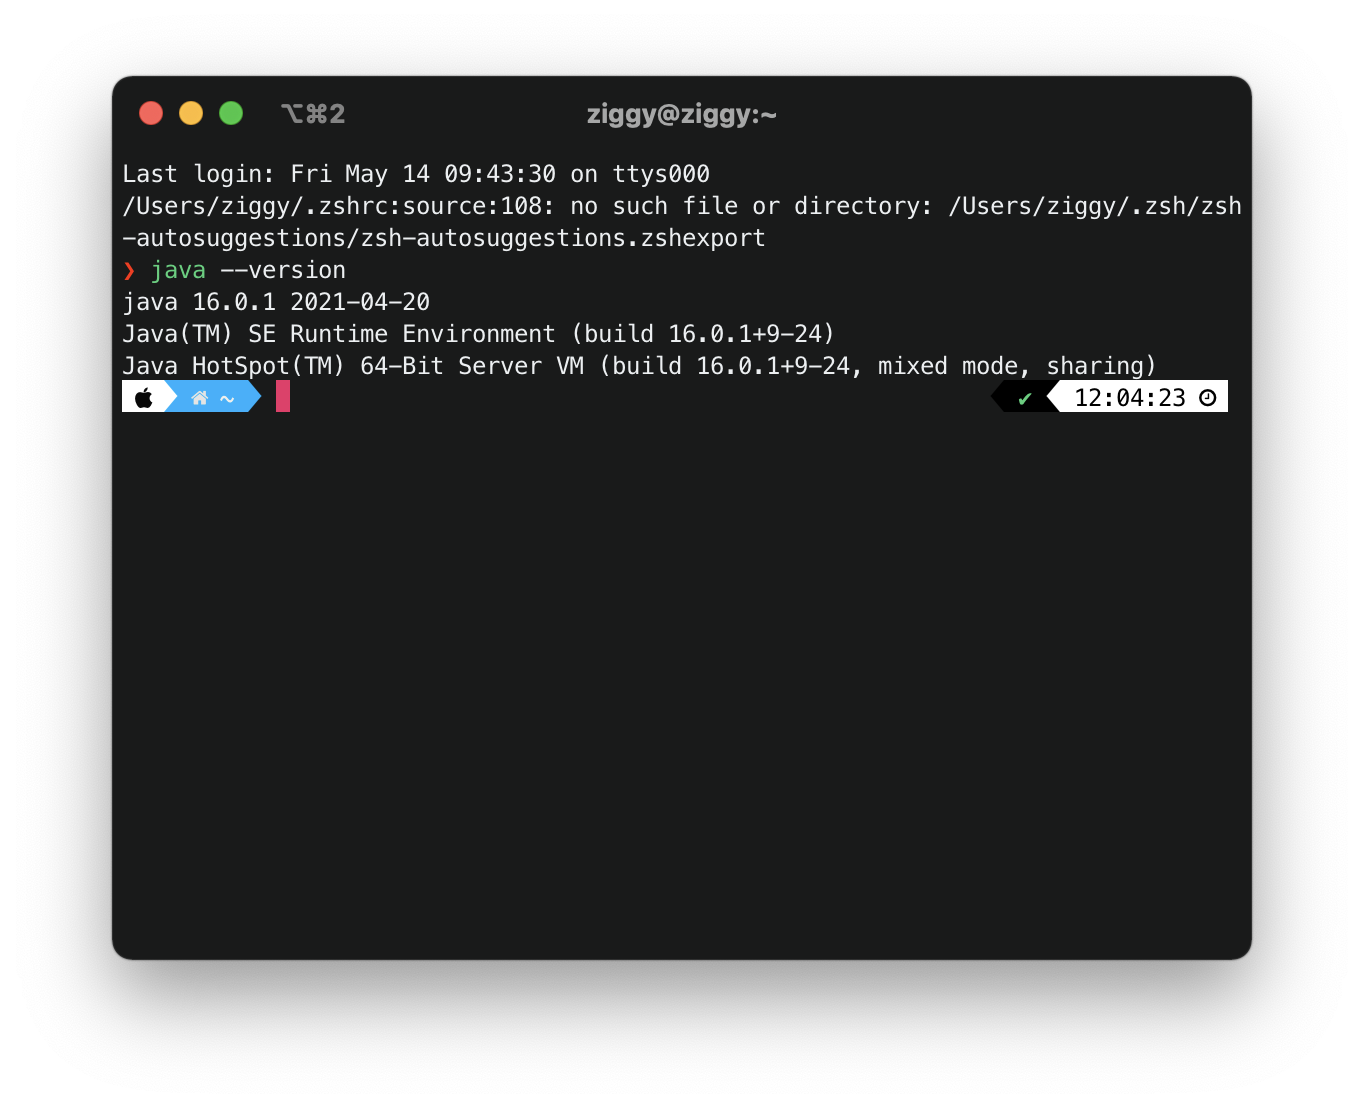
\includegraphics[width=10cm]{img/jdk-version.png}
        \caption{De terminal bevestigd dat Java SE 16 correct is geïnstalleerd op de betreffende computer}
        \label{fig:M-jdk-version}
    \end{figure}

\section{\IfLanguageName{dutch}{Basis Kotlin Multiplatform Mobile applicatie}{Basic Kotlin MultiPlatforn Mobile application}}
\label{sec:M-first-app}
Nadat alle software is geïnstalleerd kan er overgegaan worden naar de eerste Kotlin Multiplatform Mobile applicatie (KMM). De eerste applicatie zal een kleine applicatie zijn die aan de gebruiker zal tonen welke software versie op het toestel geïnstalleerd staat.
\\ \\
De geschreven applicatie kan ook op GitHub\footnote{github.com} teruggevonden worden. Dit kan via volgende link:\\
\verb*|https://github.com/ziggymoens/KMM_Application_Basic|
\\ \\
Bij het opstarten van Android Studio geeft deze de optie om een nieuw project te starten, eens dat is aangeklikt wordt er gekozen voor de optie `KMM Application'. Als naam wordt `Basic KMM Application' gekozen en hierbij wordt de minimum SDK op level 28 gezet (Android 9.0\footnote{android.com/versions/pie-9-0})

\begin{figure}
    \centering
    \subfloat[\centering Startscherm Android Studio]{{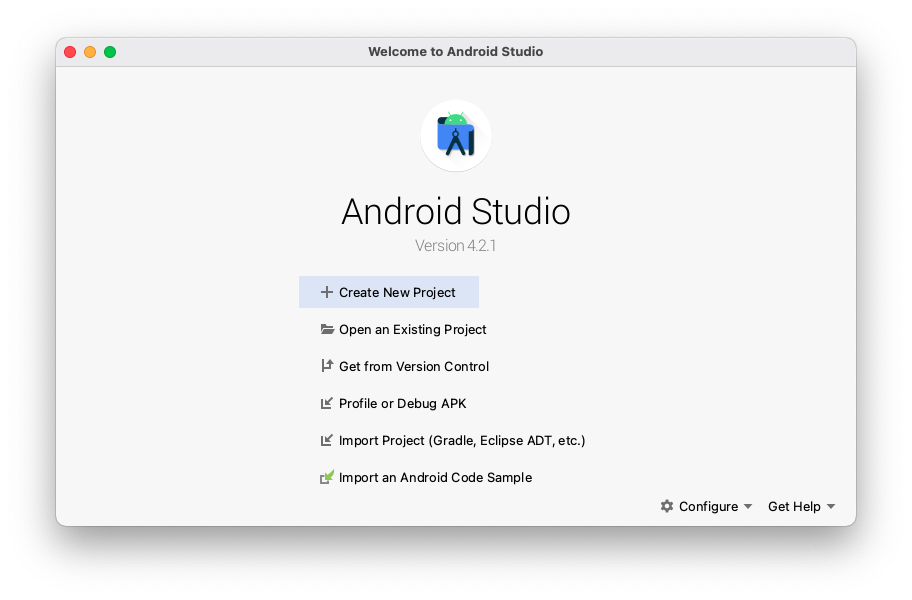
\includegraphics[width=7cm]{img/kmm-start-1} }}
   
    \subfloat[\centering Nieuw project met de KMM application optie]{{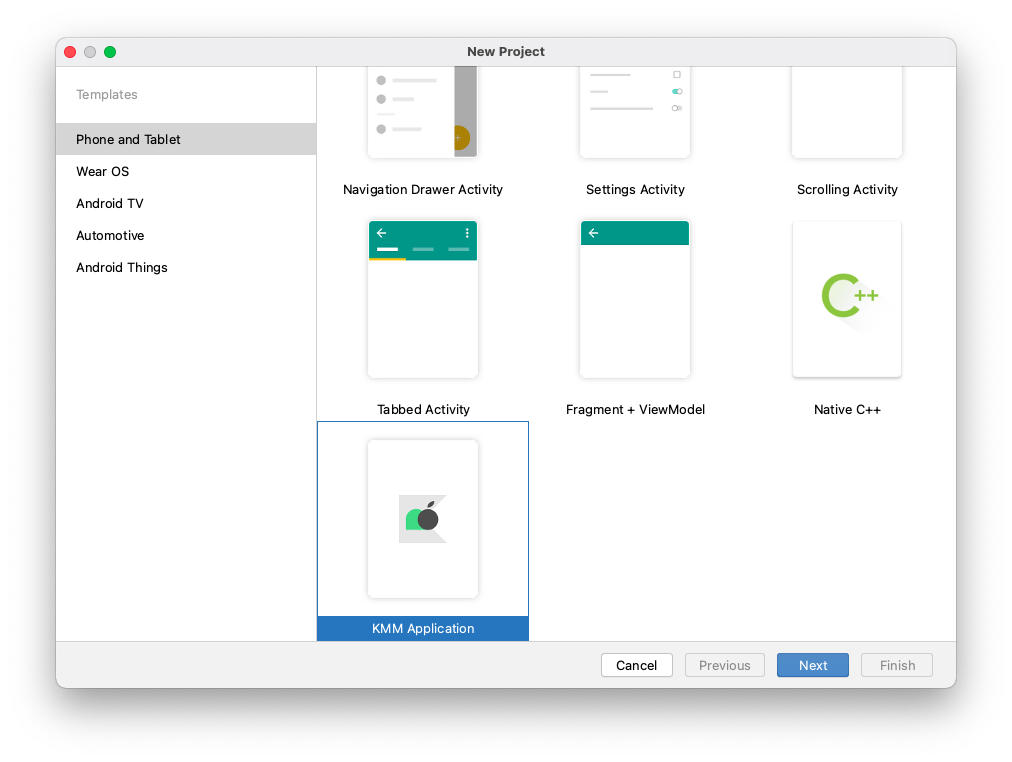
\includegraphics[width=7cm]{img/kmm-start-2} }}
    
    \subfloat[\centering Standaard instellingen Android Project]{{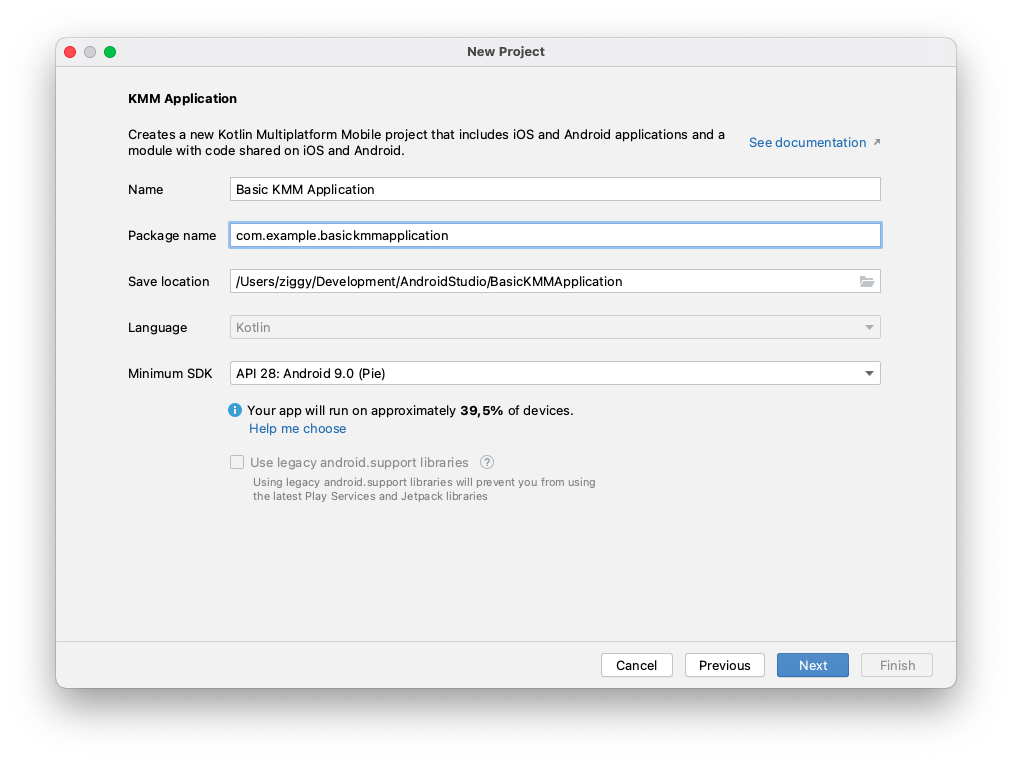
\includegraphics[width=7cm]{img/kmm-start-3} }}
    
    \subfloat[\centering Specifieke KMM project instellingen]{{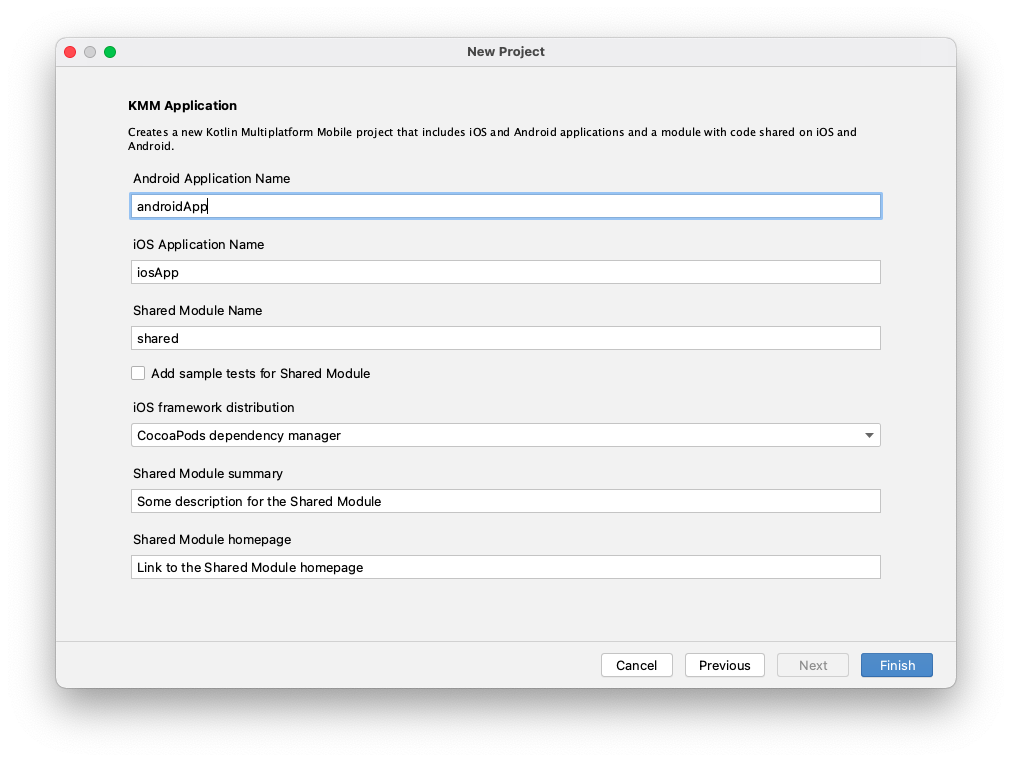
\includegraphics[width=7cm]{img/kmm-start-4} }}
    \caption{Proces voor het opzetten van een KMM project}
    \label{fig:M-kmm-startup}%
\end{figure}

Eens het project correct is ingeladen en geïndexeerd kan gezien worden dat het project al standaard de code bevat om een gebruiker zijn software versie te tonen. Daarnaast zal de KMM plugin binnen Android Studio de juiste omgevingen aanmaken om de code te draaien/testen binnen de juiste emulators. 

\begin{figure}
    \centering
    \subfloat[\centering Instellingen Android emulator]{{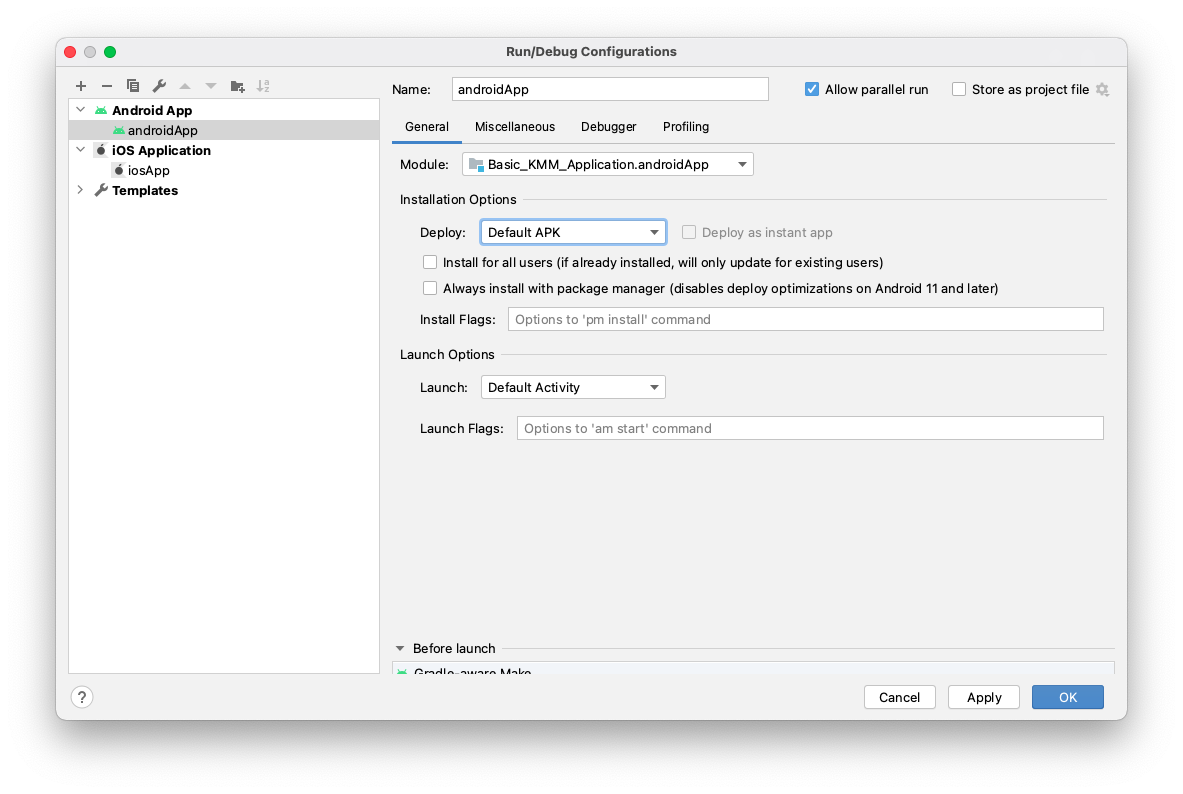
\includegraphics[width=8cm]{img/as-emulators-1} }}
    
    \subfloat[\centering Instellingen iOS emulator]{{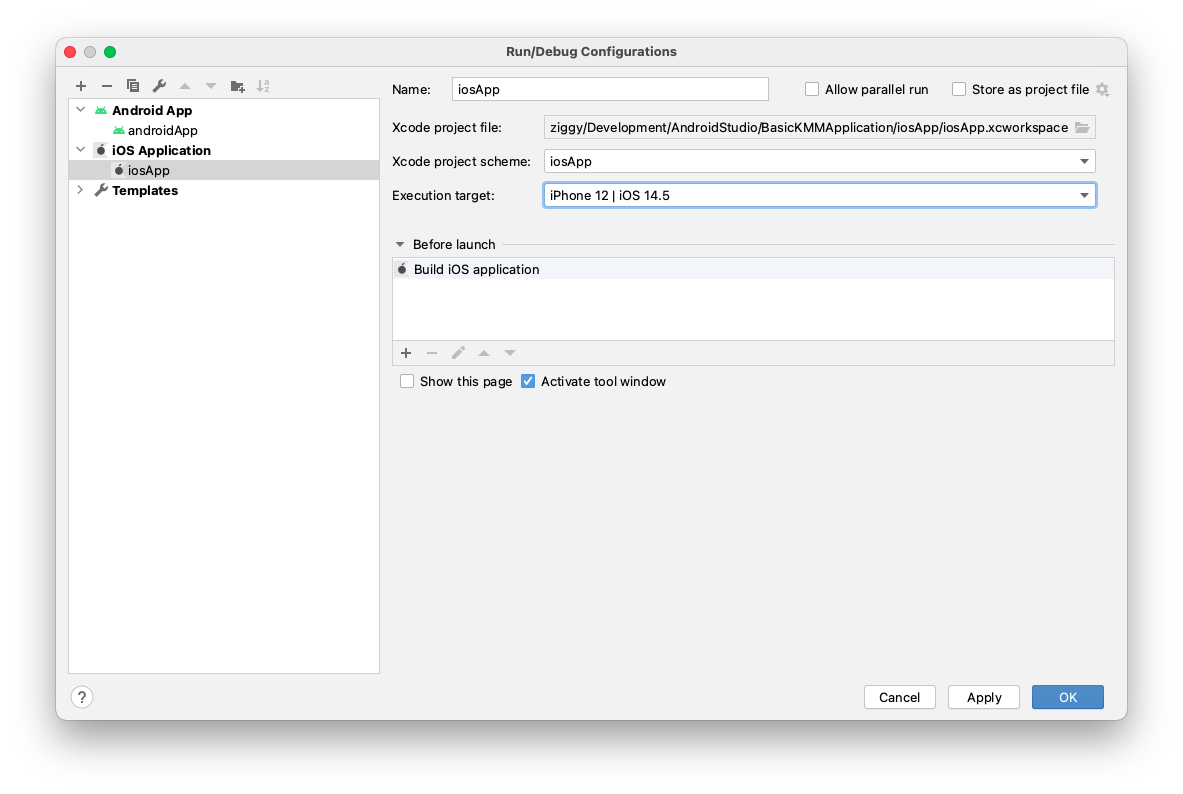
\includegraphics[width=8cm]{img/as-emulators-2} }}
    
    \caption{Android en iOS emulators binnen Android Studio}
    \label{fig:M-as-emulators}
\end{figure}

Eens de emulators ingesteld zijn kan het project voor iOS en Android worden opgestart. Na 8 s 8374 ms was de Android applicatie voor de eerste keer opgestart en na 6 s 202 ms was de iOS applicatie opgestart. Hieronder een beeld van beide applicaties in actie.

\begin{figure}
    \centering
    \subfloat[\centering Android applicatie]{{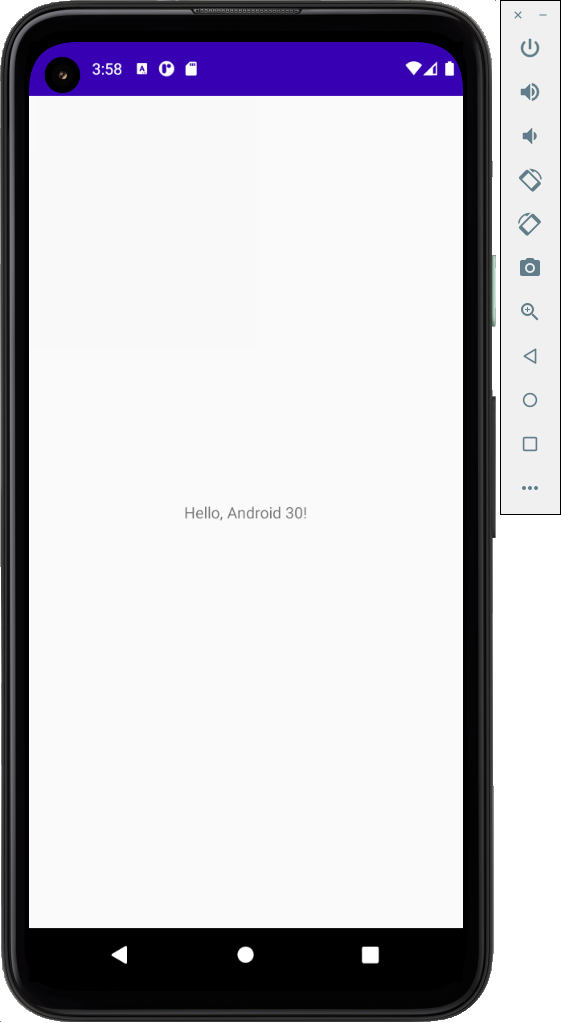
\includegraphics[width=4cm]{img/kmm-basic-android} }}
    \qquad
    \subfloat[\centering iOS applicatie]{{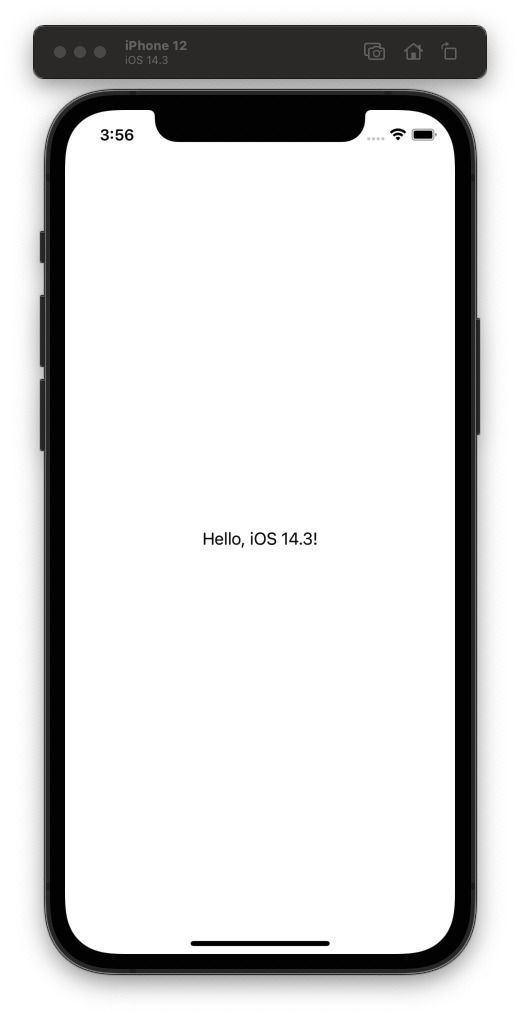
\includegraphics[width=4cm]{img/kmm-basic-ios} }}
    \caption{KMM basic applicatie op Android en iOS}
    \label{fig:M-kmm-basic}%
\end{figure}

Binnen het project kan de expect/actual structuur duidelijk teruggevonden worden. Binnen de shared-map bevindt zich de commonMain-map. Hierin zitten volgende twee bestanden.

\begin{lstlisting}
    //Greeting.kt
    
    class Greeting {
        fun greeting(): String {
            return "Hello, ${Platform().platform}!"
        }
    }
\end{lstlisting}
\begin{lstlisting}
    //Platform.kt
    
    expect class Platform() {
        val platform: String
    }
\end{lstlisting}

Ook in de shared-map kan de iosMain-map gevonden worden. Hierin komt het Platform.kt bestand nogmaals terug. Hierbij wordt echter de `expect' geïmplementeerd en verwerkt in de `actual'. 

\begin{lstlisting}
    //Platform.kt
    
    actual class Platform actual constructor() {
        actual val platform: String = 
            UIDevice.currentDevice.systemName() + 
            " " + 
            UIDevice.currentDevice.systemVersion
    }
\end{lstlisting}

De laatste map binnen de shared-map die interessant is voor deze studie is de androidMain-map en hierin wordt ook de Platform.kt verwerkt.

\begin{lstlisting}
    //Platform.kt
    
    actual class Platform actual constructor() {
        actual val platform: String = 
            "Android ${android.os.Build.VERSION.SDK_INT}"
    }
\end{lstlisting}

Zoals duidelijk zichtbaar zal in de shared-map de globale structuur worden vastgelegd en deze zal dan verwerkt worden binnen de platform specifieke delen.

Uiteindelijk zal de Greetings klasse worden opgeroepen binnen de Android en iOS applicaties zoals hieronder geïllustreerd
\begin{lstlisting}
    //Android - MainActivity.kt
    
    fun greet(): String {
        return Greeting().greeting()
    }
\end{lstlisting}
\begin{lstlisting}
    //iOS - ContentView.swift
    
    struct ContentView: View {
       let greet = Greeting().greeting()
       
       var body: some View {
           Text(greet)
       }
    }
   
\end{lstlisting}

\section{\IfLanguageName{dutch}{Basis native applicaties}{Basic native applications}}
\label{sec:M-first-native}
Nu de KMM applicatie gemaakt is, kan de native variant voor Android en iOS gemaakt worden. Hierbij zal geprobeerd worden deze zo goed mogelijk op elkaar af te stemmen.
\\ \\
De geschreven applicaties kunnen ook op GitHub\footnote{github.com} teruggevonden worden. Dit kan via volgende links:\\
\textbf{Android}:
\\ \\
\verb*|https://github.com/ziggymoens/Android_Native_Basic|
\\ \\
\textbf{iOS}:\\
\verb*|https://github.com/ziggymoens/iOS_Native_Basic|
\\ \\

\subsection{\IfLanguageName{dutch}{Android}{Android}}
\label{sec:M-first-native-android}


 \begin{figure}
    \centering
    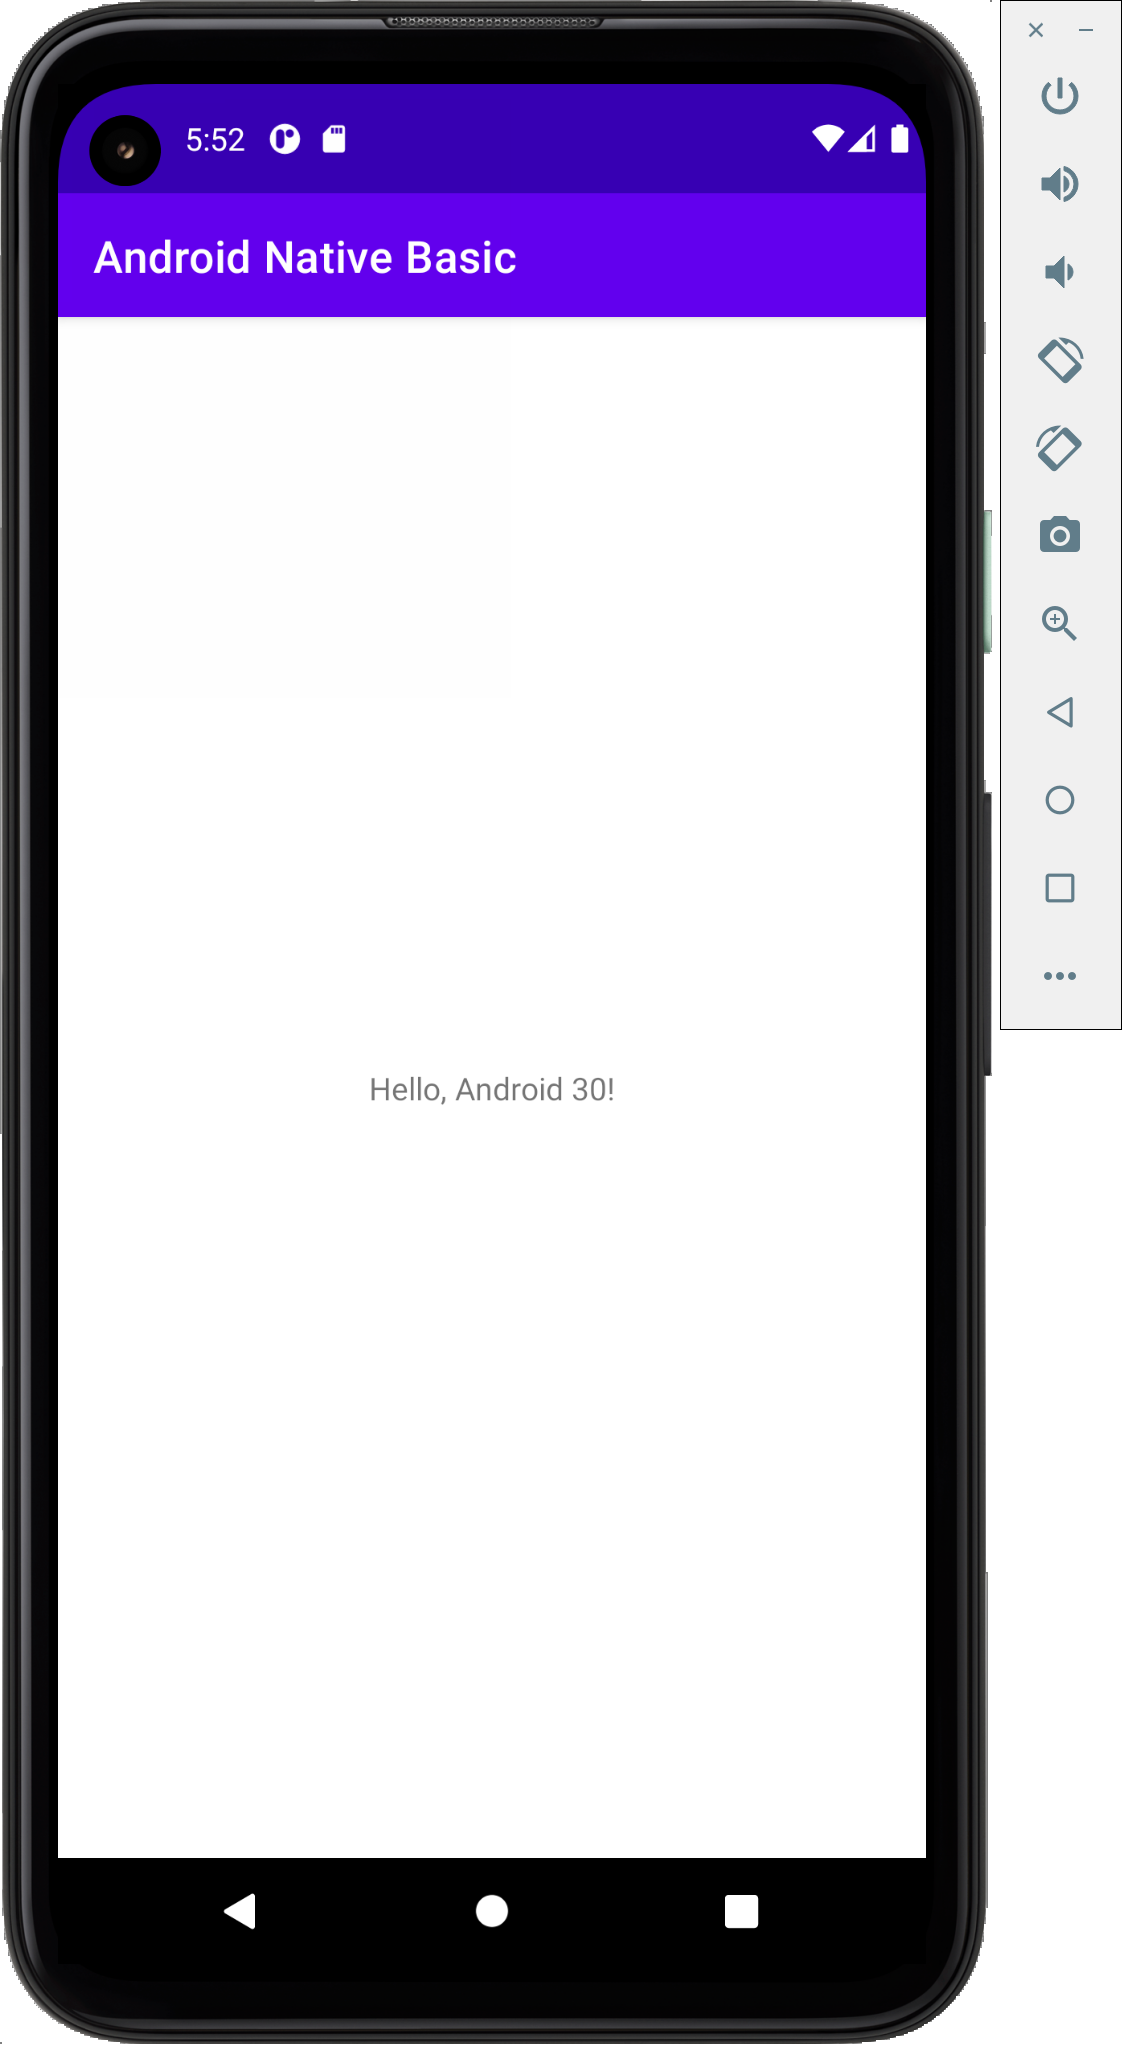
\includegraphics[width=7cm]{img/android-basic.png}
    \caption{Interface van de basic Android applicatie}
    \label{fig:M-basic-android}
\end{figure}

\begin{lstlisting}
    //MainActivity.kt
    
    class MainActivity : AppCompatActivity() {
        
        override fun onCreate(savedInstanceState: Bundle?) {
            super.onCreate(savedInstanceState)
            setContentView(R.layout.activity_main)
            
            val tv: TextView = findViewById(R.id.text_view)
            tv.text = "Hello, Android ${android.os.Build.VERSION.SDK_INT}!"
        }
    }
    
    
    //activity_main.xml
    
    <?xml version="1.0" encoding="utf-8"?>
    <androidx.constraintlayout.widget.ConstraintLayout xmlns:android="http://schemas.android.com/apk/res/android"
       xmlns:app="http://schemas.android.com/apk/res-auto"
       xmlns:tools="http://schemas.android.com/tools"
       android:id="@+id/main_view"
       android:layout_width="match_parent"
       android:layout_height="match_parent">
    
       <TextView
           android:id="@+id/text_view"
           android:layout_width="wrap_content"
           android:layout_height="wrap_content"
           app:layout_constraintBottom_toBottomOf="parent"
           app:layout_constraintLeft_toLeftOf="parent"
           app:layout_constraintRight_toRightOf="parent"
           app:layout_constraintTop_toTopOf="parent"
           tools:text="Hello World!" />
                
    </androidx.constraintlayout.widget.ConstraintLayout>
\end{lstlisting}

\subsection{\IfLanguageName{dutch}{iOS}{iOS}}
\label{sec:M-first-native-ios}

 \begin{figure}
    \centering
    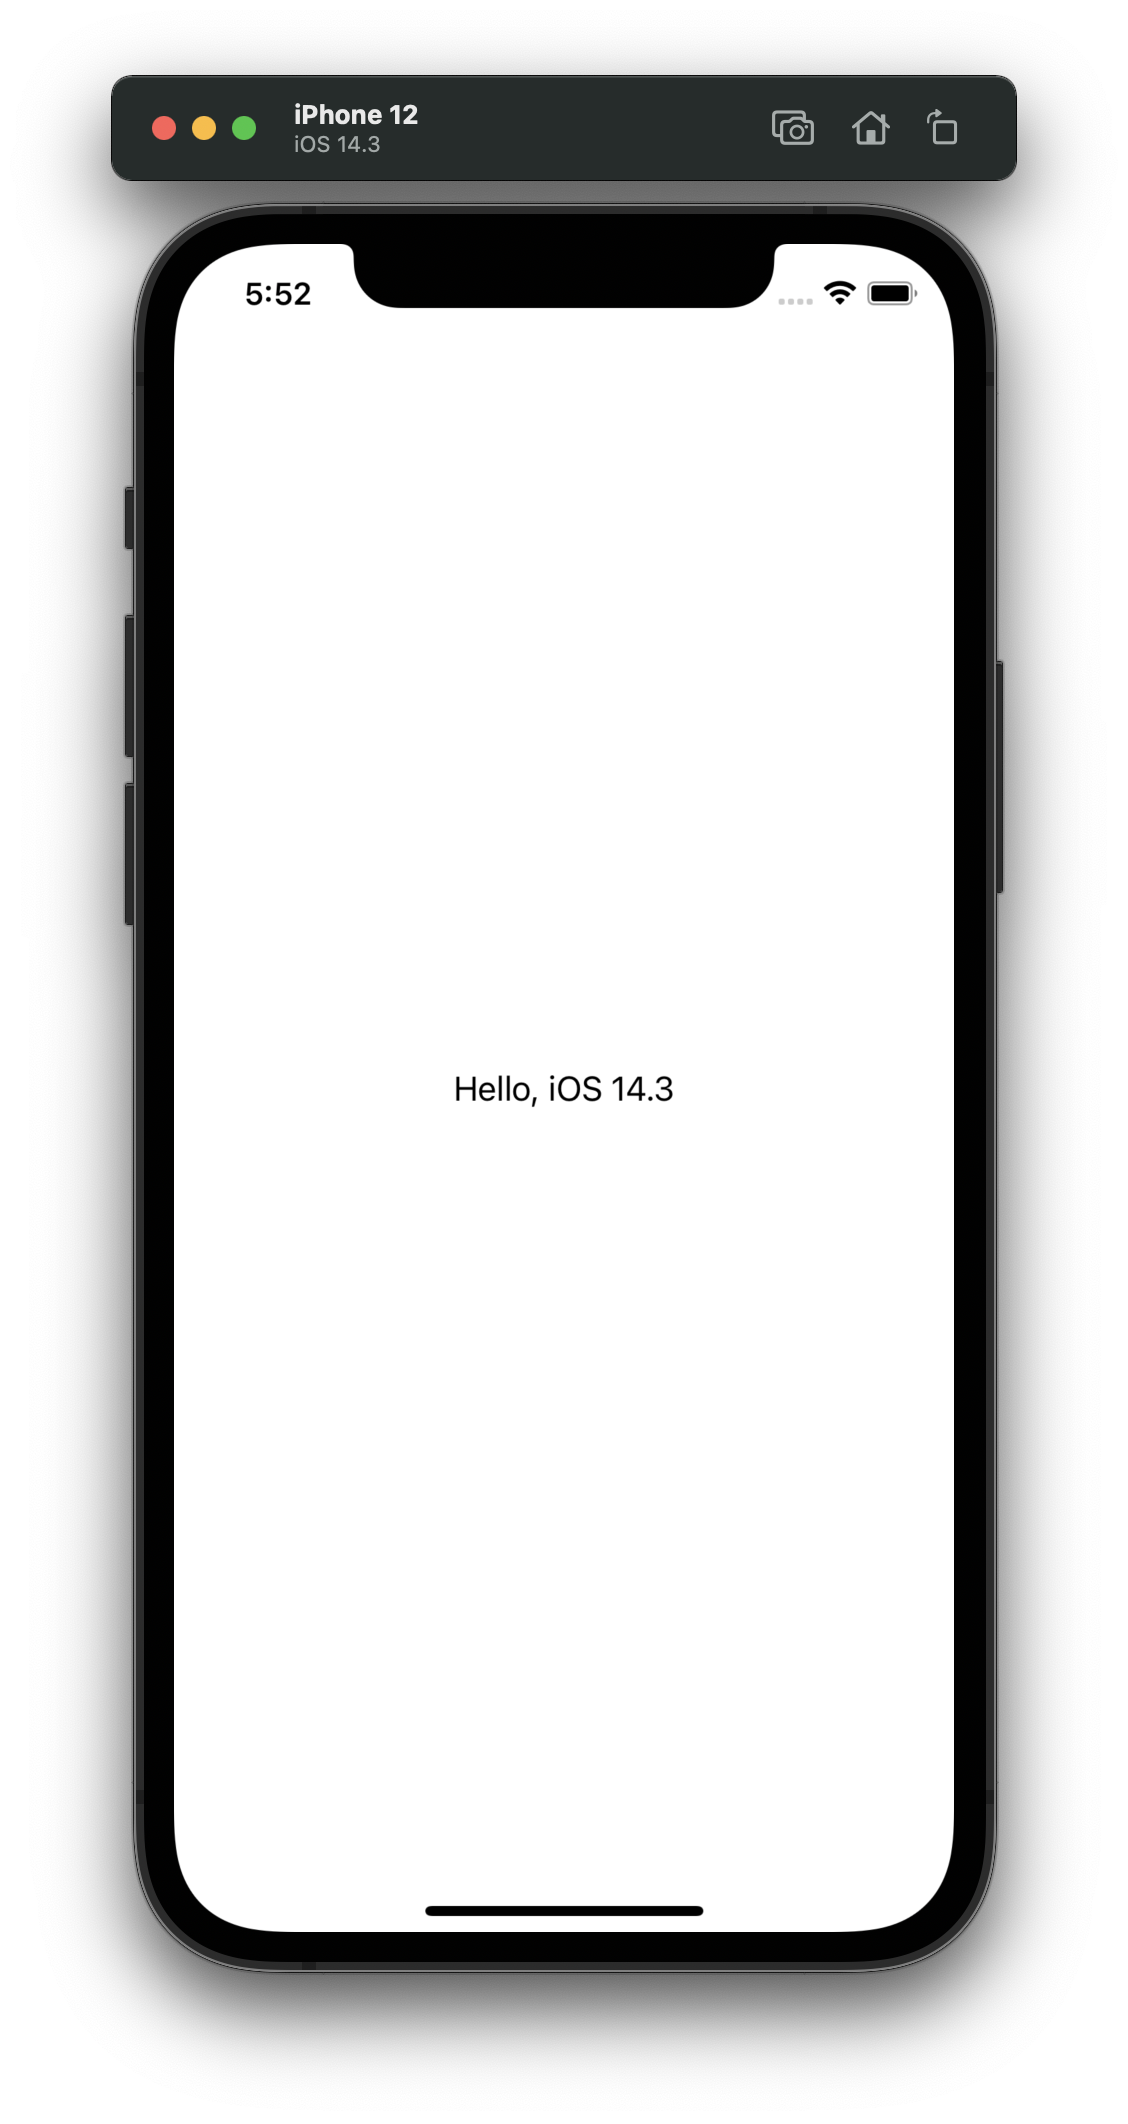
\includegraphics[width=7cm]{img/ios-basic.png}
    \caption{Interface van de basic iOS applicatie}
    \label{fig:M-basic-ios}
\end{figure}


\begin{lstlisting}
    // ViewController.swift
    
    class ViewController: UIViewController {
        
        @IBOutlet weak var label: UILabel!
        
        override func viewDidLoad() {
            super.viewDidLoad()
            
            label.text = "Hello, " + UIDevice.current.systemName + " " + UIDevice.current.systemVersion
        }
    }
    
\end{lstlisting}

